\documentclass[12pt,a4paper]{report}
\usepackage[top=2.5cm, bottom=2.5cm, left=2.5cm, right=2.5cm]{geometry}
\usepackage[utf8]{inputenc}
\usepackage[T1]{fontenc}%              gestion des accents (PDF)
\usepackage[french,english]{babel}%          gestion du français
\usepackage{fancyhdr}
\usepackage[pdftex]{graphicx}
\usepackage{setspace}
\usepackage{hyperref}
\usepackage[french]{varioref}
\usepackage{color}
\usepackage{lettrine}
\usepackage{colortbl}
\usepackage{amsmath}
\usepackage{ifpdf} %part of the hyperref bundle
\usepackage{array}
\usepackage{nicefrac}
\usepackage{tabularx}
\usepackage{abstract}
\usepackage{tikz}
\usepackage[pages=some]{background}
\usepackage{siunitx}
\usepackage{float}
\usepackage{stmaryrd}
\usepackage{tikz}
\usetikzlibrary{calc}



\usepackage{romannum}
\usepackage[utf8]{inputenc}
\usepackage[T1]{fontenc}
\usepackage[french]{babel}
\frenchbsetup{StandardLists=true} % à inclure si on utilise \usepackage[french]{babel}
\usepackage{enumitem}
\usepackage{amssymb}
\usepackage{cite}
%\usepackage{url}
\usepackage[resetlabels, labeled]{multibib}
\usepackage[frenchb]{babel}
\usepackage[T1]{fontenc}
\usepackage[utf8]{inputenc}
\usepackage[french]{babel}

\usepackage{listings}

\usepackage{xcolor}

\definecolor{codegreen}{rgb}{0,0.6,0}
\definecolor{codegray}{rgb}{0.5,0.5,0.5}
\definecolor{codepurple}{rgb}{0.58,0,0.82}
\definecolor{backcolour}{rgb}{0.95,0.95,0.92}

\lstdefinestyle{mystyle}{
    backgroundcolor=\color{backcolour},
    commentstyle=\color{codegreen},
    keywordstyle=\color{magenta},
    numberstyle=\tiny\color{codegray},
    stringstyle=\color{codepurple},
    basicstyle=\ttfamily\small,
    breakatwhitespace=false,
    breaklines=true,
    captionpos=b,
    keepspaces=true,
    numbers=left,
    numbersep=5pt,
    showspaces=false,
    showstringspaces=false,
    showtabs=false,
    tabsize=2
}

\lstset{style=mystyle}







\usepackage{xurl}
\usepackage{breakurl}

\usepackage{hyperref}


\newcites{ref}{Webographie}

 % set fonts for nicer pdf view
\linespread{1.5}
\IfFileExists{lmodern.sty}{\usepackage{lmodern}}{}
\fancypagestyle{noheadrule}{
\fancyhf{}
\renewcommand{\headrulewidth}{0pt}
\renewcommand{\footrulewidth}{0pt}
\fancyfoot[LE,LO]{\textit {Report}}
\fancyfoot[RE,RO]{\bfseries\thepage}
}
\setcounter{secnumdepth}{4}
\setcounter{tocdepth}{4}


%\setcounter{secnumdepth}{4}
% Début du document
\begin{document}
\include{Page_de_garde}
\null\thispagestyle{empty}
%\include{Page_de_garde2}
%\null\thispagestyle{empty}
%\include{garde_sign_fin}
\renewcommand{\chaptermark}[1]{\markboth{Chapitre~\thechapter~:~#1}{}}
\fancyhf{}
\pagestyle{fancy}
\fancyhead[RE,RO]{\bfseries\leftmark}
\fancyfoot[LE,LO]{\textit{}}
\fancyfoot[RE,RO]{\bfseries\thepage}
\fancypagestyle{plain}{
\fancyhead{}
\renewcommand{\headrulewidth}{0pt}
}


\newpage
\pagenumbering{gobble}
\include{resume}
\include{Dedicace}
\include{Remerciements}
\include{fiche}
\include{Abstract}


\selectlanguage{french}

\tableofcontents % Table des matières
\newpage
\pagenumbering{arabic}
\chapter*{Introduction}
\addcontentsline{toc}{chapter}{Introduction générale}
%\setlength{\parindent}{2cm} 
%\setlength{\parindent}{1cm}
\hspace{0.58cm}
Les séries temporelles sont des données qui sont collectées au fil du temps et qui sont
organisées de manière chronologique. Elles peuvent être utilisées pour analyser et comprendre les tendances et les modèles dans les données au fil du temps, ainsi que pour faire des prévisions sur les événements futurs. Les séries temporelles peuvent être trouvées dans de nombreux domaines, tels que la finance, l’économie, la météorologie, la santé...\\

Les modèles de rupture, également connus sous le nom de modèles de changement de régime, sont des outils statistiques qui permettent de détecter et de modéliser les changements dans la structure d’une série temporelle. Ces modèles sont souvent utilisés pour analyser des données économiques, financières, météorologiques ou sociales, où il peut y avoir des périodes de stabilité suivies de périodes de changement soudain.\\

Les modèles de rupture permettent d’identifier les moments où un changement significatif s’est produit dans les données et de modéliser le comportement de la série temporelle avant et après ce changement. Autrement dit, pour une séquence donnée de variables aléatoires $(X_i)_{1\leq i\leq n}$, nous essayons de trouver un point de rupture $k$ où les éléments $X_1, ..., X_k$ ont une fonction de distribution identique $f_1$ et les éléments $X_{k+1}, ..., X_n$ sont distribuées selon une autre densité de probabilité $f_2$.\\

Dans le rapport qui suit nous allons nous pencher sur le Modèle de Rupture pour la loi normale asymétrique (Skew normal distribution) et l’appliquer aux données mensuelles de TER.\\




\chapter{Contextualisation}
\markboth{CHAPITRE 1. Contextualisation}{

\section{Présentation des données}

Notre jeu de données contient les informations relatives aux TER en circulation dans différentes régions de France. Ces informations sont mensuelles, et nous disposons d'un nombre d'observations différent selon la région concernée (\textit{cf Figure 1.1}).\\

\begin{figure}[H]
  \centering
  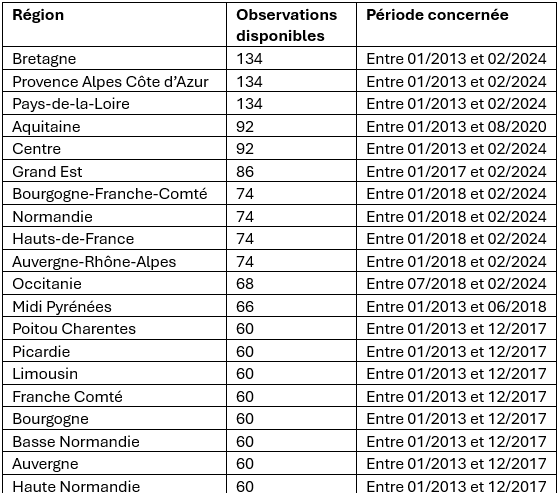
\includegraphics[width=0.8\textwidth]{Tableau_1_1.png}
\end{figure}

\begin{figure}[H]
  \centering
  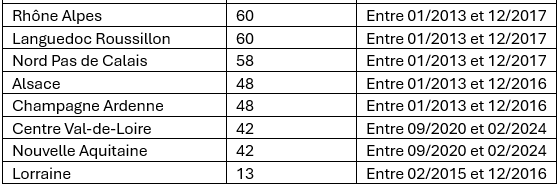
\includegraphics[width=0.8\textwidth]{Tableau_1_2.png}
  \caption{Nombre d'observations en fonction de la région}
\end{figure}

Dans notre rapport, nous considérons seulement les régions pour lesquelles nous avons plus de 70 observations (les autres régions sont traitées dans le code joint au rapport). Pour chacune de  ces régions, nous nous intéressons en particulier aux variables \textbf{'nombre de trains programmés'} et\textbf{ 'nombre de trains annulés'}. Ces variables constituent des séries temporelles auxquelles nous appliquerons notre modèle de rupture.

\section{Modèle de rupture}

Nous souhaitons appliquer notre modèle de rupture aux séries temporelles correspondant au nombre de trains programmés et au nombre de trains annulés pour les régions sélectionnées.\\

Nous utilisons un \textbf{modèle de rupture pour la loi normale asymétrique}. La densité de la loi normale asymétrique est de la forme:
\[
f(x,\mu,\sigma,\theta) = \frac{2\phi\left(\frac{x-\mu}{\sigma}\right)\Phi\left(\theta\left(\frac{x-\mu}{\sigma}\right)\right)}{\sigma}
\]
où $\phi(x) = \frac{1}{\sqrt{2\pi}}e^{-\frac{x^2}{2}}$ et $\Phi(x) = \int_{-\infty}^{x} \phi(t)dt$.\\

Nous considérons le modèle suivant :
\[
\begin{cases}
X_t \sim \mathcal{SN}(\mu_1,\sigma_1,\theta) & \text{si } t \leq k \\
X_t \sim \mathcal{SN}(\mu_2,\sigma_2,\theta) & \text{si } t > k
\end{cases}
\]
où $\mu_1$, $\sigma_1$, $k$, $\mu_2$, $\sigma_2$, $\theta$ sont inconnus que l'on souhaite estimer.\\

Concrètement, nous suivons la démarche suivante:

\begin{itemize}
  \item Soit k, un moment de rupture supposé. Nous évaluons les paramètres des lois normales asymétriques des variables aléatoire $X_1, ..., X_k$ et $X_{k+1}, ..., X_n$ en nous basant sur les échantillons dont nous disposons.
  \item Nous souhaitons déterminer $\hat{k}$, le moment de rupture le plus probable. Pour cela, nous évaluons les paramètres des lois normales asymétrique pour chaque k candidat (c'est à dire appartenant à $\llbracket 10, n-10 \rrbracket$ ). Nous sélectionnons alors k tel que les lois obtenues en considérant ce moment de rupture soient le plus plausible.
  \item Ayant déterminé $\hat{k}$, nous testons la similarité en loi des échantillons ($x_1, ..., x_{\hat{k}}$) et ($x_{\hat{k}+1}, ..., x_n$).
\end{itemize}

La mise en œuvre de chaque étape est détaillée dans le chapitre suivant.


}



\chapter{Méthode de detection du point de rupture}
    %\addcontentsline{toc}{chapter}{}
\markboth{CHAPITRE 2. Méthode de detection du point de rupture}{

La détection de point de rupture est une tâche cruciale dans de nombreux domaines tels que l'économie, la météorologie et la surveillance de processus industriels. Identifier avec précision ces points peut révéler des éléments importants sur les événements sous-jacents ou les changements de régime.\\

La méthode utilisée dans notre analyse repose sur la maximisation de la vraisemblance, une approche robuste qui consiste à ajuster les paramètres de modèles statistiques de manière à rendre la séquence de données observées aussi probable que possible sous ces modèles. Cette méthode est particulièrement efficace pour modéliser des séries avec des ruptures, car elle permet de comparer rigoureusement les hypothèses de continuité contre celles de changement à des instants spécifiques.

\section{Estimation des paramètres pour un point de rupture donné}

Soit k\in  $\llbracket 10, n-10 \rrbracket$ , un point de rupture supposé. On a alors:\\

\[
\begin{cases}
$X_1, ..., X_k$ \sim \mathcal{SN}(\mu_1,\sigma_1,\theta)  \\
$X_{k+1}, ..., X_n$ \sim \mathcal{SN}(\mu_2,\sigma_2,\theta)
\end{cases}
\]
Sous hypothèse d'indépendance des observations, la vraisemblance s'écrit alors:\\

L($\underline{x}$,\mu_1,\mu_2,\sigma_1,\sigma_2,\theta)= $\displaystyle{\prod_{i=1}^k f_{1}(x_i,\mu_1,\sigma_1,\theta)}$ * $\displaystyle{\prod_{i=k+1}^n f_{2}(x_i,\mu_2,\sigma_2,\theta)}$ \\
où 

\[
\begin{cases}
f_{1}(x_i,\mu_1,\sigma_1,\theta)= \frac{2\phi\left(\frac{x_i-\mu_1}{\sigma_1}\right)\Phi\left(\theta\left(\frac{x_i-\mu_1}{\sigma_1}\right)\right)}{\sigma_1}  \\
f_{2}(x_i,\mu_2,\sigma_2,\theta)= \frac{2\phi\left(\frac{x_i-\mu_2}{\sigma_2}\right)\Phi\left(\theta\left(\frac{x_i-\mu_2}{\sigma_2}\right)\right)}{\sigma_2}
\end{cases}
\]

soit: \\

L($\underline{x}$,\mu_1,\mu_2,\sigma_1,\sigma_2,\theta)=\frac{2^n}{\sigma_1^k*\sigma_2^{(n-k)}}*$\displaystyle{\prod_{i=1}^k \phi(\frac{x_i-\mu_1}{\sigma_1})*\Phi(\theta(\frac{x_i-\mu_1}{\sigma_1})) }$*$\displaystyle{\prod_{i=k+1}^n \phi(\frac{x_i-\mu_2}{\sigma_2})*\Phi(\theta(\frac{x_i-\mu_2}{\sigma_2})) }$\\

Pour simplifier les calculs, nous passons à la log vraisemblance et nous obtenons finalement:\\


{\center 
l($\underline{x}$,\mu_1,\mu_2,\sigma_1,\sigma_2,\theta)=\\
$\frac{n}{2}$*log(2)-$\frac{n}{2}*$log(\pi)-k*log(\sigma_1)-(n-k)*log(\sigma_2)-\frac{1}{2*\sigma_1^2}*$\displaystyle{\sum_{i=1}^k (x_i-\mu_1)^2}$\\
+$\displaystyle{\sum_{i=1}^k log(\Phi(\theta(\frac{x_i-\mu_1}{\sigma_1})))}$
-$\frac{1}{2*\sigma_2^2}$*$\displaystyle{\sum_{i=k+1}^n (x_i-\mu_2)^2}$+$\displaystyle{\sum_{i=k+1}^n log(\Phi(\theta(\frac{x_i-\mu_2}{\sigma_2})))}$
}

\vspace{1cm}

\textit{Ou encore}

{\center 
l($\underline{x}$,\mu_1,\mu_2,\sigma_1,\sigma_2,\theta)=\\
C^{te}-k*log(\sigma_1)-(n-k)*log(\sigma_2)-\frac{1}{2*\sigma_1^2}*$\displaystyle{\sum_{i=1}^k (x_i-\mu_1)^2}$+$\displaystyle{\sum_{i=1}^k log(\Phi(\theta(\frac{x_i-\mu_1}{\sigma_1})))}$\\
-$\frac{1}{2*\sigma_2^2}$*$\displaystyle{\sum_{i=k+1}^n (x_i-\mu_2)^2}$+$\displaystyle{\sum_{i=k+1}^n log(\Phi(\theta(\frac{x_i-\mu_2}{\sigma_2})))}$
}

\vspace{1cm}

On peut alors estimer les paramètres des deux lois normales asymétriques par maximisation de la log vraisemblance:\\

 $\hat{\mu_1}^k$,$\hat{\mu_2}^k$,$\hat{\sigma_1}^k$,$\hat{\sigma_2}^k$,$\hat{\theta}^k$ \hspace{0.05cm}=\hspace{0.05cm}argmax_{\mu_1,\mu_2,\sigma_1,\sigma_2,\theta} \hspace{0.1cm}l($\underline{x}$,\mu_1,\mu_2,\sigma_1,\sigma_2,\theta)\\
 
sous conditions $\sigma_1$, $\sigma_2$>0 \\

Si nous calculons les dérivées partielles de la log vraisemblance , nous nous rendons compte qu'il n'existe pas de solution explicite. Nous utiliserons donc la fonction minimize du module scipy.optimize sur l'opposé de la log vraisemblance afin de pouvoir estimer les paramètres des lois. \\

Le code de la fonction permettant d'estimer les paramètres des lois pour un point de rupture donné est fourni en \textbf{ANNEXE}

\section{Détermination de $\hat{k}$, point de rupture optimal}

À présent, nous voulons déterminer $\hat{k}$, le point de rupture optimal, parmi les points de rupture candidats k \in  $\llbracket 10, n-10 \rrbracket$\\

Pour cela, pour chaque k candidat, nous estimons les paramètres des lois normales asymétriques en utilisant la méthode décrite dans la section précédente: nous obtenons alors $\hat{\mu_1}^k$,$\hat{\mu_2}^k$,$\hat{\sigma_1}^k$,$\hat{\sigma_2}^k$,$\hat{\theta}^k$ pour chaque k.\\
Nous pouvons alors calculer la log vraisemblance en fonction de k en utilisant ces paramètres estimés:\\
\Lambda(k)=l($\underline{x}$,$\hat{\mu_1}^k$,$\hat{\mu_2}^k$,$\hat{\sigma_1}^k$,$\hat{\sigma_2}^k$,$\hat{\theta}^k$)\\

Une fois encore, nous cherchons à maximiser la vraisemblance et le point de rupture se trouve de la manière suivante:

$\hat{k}$=\hspace{0.05cm}argmax_{k} \hspace{0.1cm}\Lambda(k)\\

Le code de la fonction permettant de trouver le point de rupture optimal est donné en \textbf{ANNEXE}

\section{Test de Kolmogorov-Smirnov}

Ayant trouvé $\hat{k}$, nous nous interrogons sur la pertinence d'un tel point de rupture et donc sur la nécessité de séparer l'échantillon ($x_1, ..., x_{\hat{k}}$,$x_{\hat{k}+1},..., x_n$) en deux sous échantillons ($x_1, ..., x_{\hat{k}}$,) et ($x_{\hat{k}+1}, ..., x_n$). Pour cela nous cherchons à tester la similarité en loi des échantillons ($x_1, ..., x_{\hat{k}}$,) et ($x_{\hat{k}+1}, ..., x_n$). Nous utiliserons le test de \textbf{Kolmogorov-Smirnov}.\\

Le test de Kolmogorov-Smirnov est un test d'hypothèse statistique permettant de tester la similarité en loi de deux échantillons. Autrement dit, il permet de tester si deux échantillons ont été générés ou non par la même loi.

\[
\begin{cases}
H_0: Les\hspace{0.1cm}deux\hspace{0.1cm} échantillons\hspace{0.1cm} sont\hspace{0.1cm} générés\hspace{0.1cm} par\hspace{0.1cm} la\hspace{0.1cm} même\hspace{0.1cm} loi \\
H_1: Les\hspace{0.1cm} deux\hspace{0.1cm} échantillons\hspace{0.1cm} sont\hspace{0.1cm} générés\hspace{0.1cm} par\hspace{0.1cm} deux\hspace{0.1cm} lois\hspace{0.1cm} différentes
\end{cases}
\]\\

Nous utiliserons la p-value du test avec un seuil de confiance $\alpha$=0.05

\begin{itemize}
  \item \textbf{p-value<$\alpha$}: on rejette $H_0$. Il y a des preuves suffisantes pour affirmer que les deux échantillons ont été générés par deux lois différentes.
  \item \textbf{p-value$\geq$ $\alpha$}: on ne rejette pas $H_0$. Il n'y a pas de preuves suffisantes pour affirmer que les deux échantillons ont été générés par deux lois différentes.
\end{itemize}

Bien sûr, le point de rupture est pertinent seulement dans le cas de $H_1$, c'est à dire dans le cas où les deux échantillons ont été générés par deux lois différentes. \textbf{Autrement dit, le point de rupture est pertinent dans le cas où p-value<$\alpha$=0.05}\\

Pour effectuer nos test de Kolmogorov-Smirnov, mous utilisons la fonction kstest du module scipy.stats.



\chapter{Application aux données}
    %\addcontentsline{toc}{chapter}{}
\markboth{CHAPITRE 3. Application aux données}{

Nous allons à présent appliquer notre méthode de détection de point de rupture présentée au chapitre précédent à nos données.\\

Nous rappelons que dans notre rapport, nous traitons seulement les régions pour lesquelles nous disposons de plus de 70 observations (les autres régions sont traitées dans le code joint au rapport) et que notre modèle sera appliqué aux séries temporelles correspondant aux nombre de trains programmés et au nombre de trains annulés pour les régions sélectionnées (\textit{cf Figure 3.1}).

\begin{figure}[H]
  \centering
  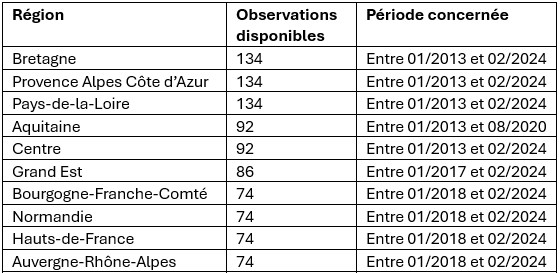
\includegraphics[width=0.8\textwidth]{Tableau_2.png}
  \caption{Régions selectionnées}
\end{figure}

\section{Bretagne}

Nous examinons la performance du réseau ferroviaire dans la région de Bretagne, en nous concentrant sur les données opérationnelles recueillies sur une période s'étendant de 2013 à 2023. Les indicateurs clés comprennent le nombre de trains programmés, ceux ayant réellement circulé, ainsi que les incidents tels que les annulations et les retards à l'arrivée.

Dans cette partie, nous avons entrepris une étude approfondie des données sur le nombre de trains programmés en Bretagne, s'étendant de 2013 à 2023. L'analyse suivante présente une visualisation de ces données, révélant les tendances sous-jacentes et les potentiels points de rupture qui ont marqué la période observée.

\subsection{Trains programmés}

Dans cette partie, nous nous concentrons sur la visualisation du nombre de trains programmés. Cette visualisation nous aide non seulement à comprendre les tendances générales et les variations saisonnières, mais elle est également cruciale pour détecter les anomalies et les points de rupture qui pourraient indiquer des changements majeurs dans la planification des transports ou refléter des réponses à des événements externes.

\begin{figure}[H]
\centering
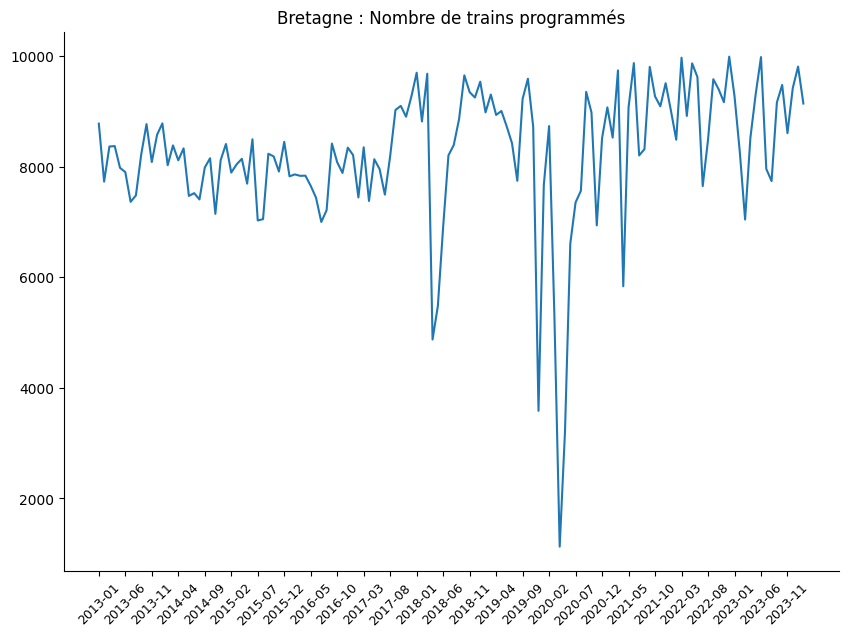
\includegraphics[width=0.8\textwidth]{image/BR-FIG1.png} 
\caption{Bretagne : Nombre de trains programmés de 2013 à 2024.}
\label{fig:trains_programmes}
\end{figure}

\begin{figure}[H]
\centering
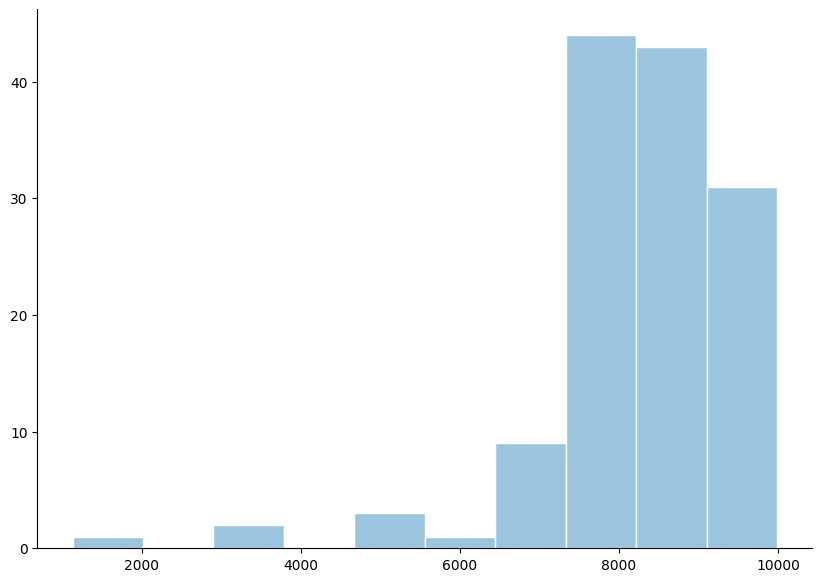
\includegraphics[width=0.8\textwidth]{image/BR-FIG2.png} 
\caption{Bretagne : Régions selectionnées.}
\label{fig:trains_programmes_2}
\end{figure}


Nous appliquons notre méthode de detection de point de rupture et nous obtenons les résultats suivants:

\subsubsection{Moment de rupture $\hat{k}$}

La date de rupture obtenue est: \textbf{2017-08}. 

\begin{figure}[H]
\centering
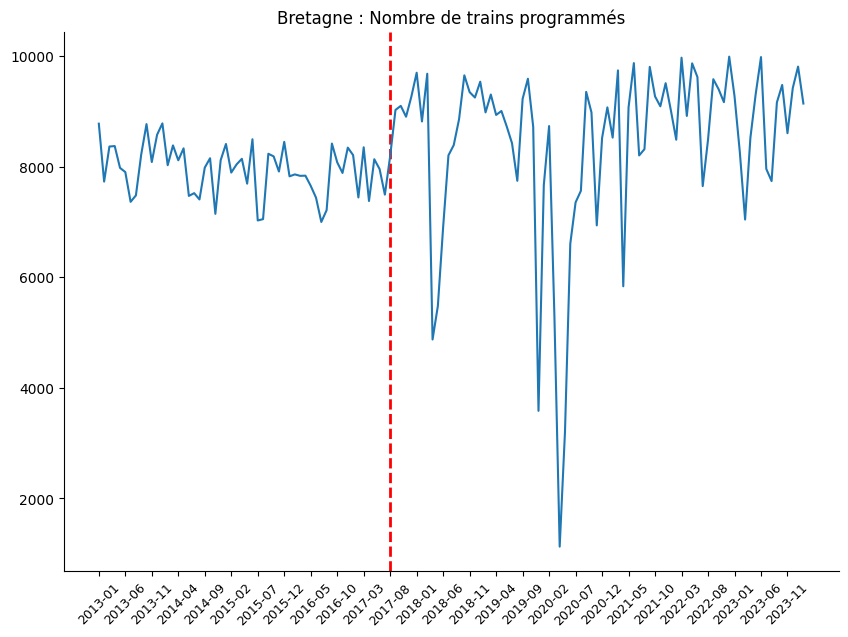
\includegraphics[width=0.8\textwidth]{image/BR-FIG4.png} 
\caption{Bretagne : La date de repture.}
\label{fig:trains_programmes_2}
\end{figure}

\subsubsection{Test de Kolmogorov-Smirnov}

Nous appliquons le test de Kolmogorov-Smirnov aux deux échantillons. Nous obtenons \textbf{p-value= 4.314571e-11}: nous rejettons $H_0$, ainsi le point de rupture est pertinent.

\subsubsection{Évaluation des paramètres des lois}

$\hat{\mu_1}^k$,$\hat{\mu_2}^k$,$\hat{\sigma_1}^k$,$\hat{\sigma_2}^k$,$\hat{\theta}^k$=( 8627.61, 9957.25, 850.73, 2140.80, -6.96)\\
 
 

Nous constatons que la moyenne des trains programmés avant le point de rupture ($\hat{\mu_1}^k$) est inférieure à celle après le point de rupture ($\hat{\mu_2}^k$). Cela indique une augmentation du nombre moyen de trains programmés post-rupture. De plus, nous observons une augmentation significative de la variance après le point de rupture ($\hat{\sigma_2}^k$ par rapport à $\hat{\sigma_1}^k$), ce qui suggère une plus grande dispersion dans le nombre de trains programmés. Ces observations sont en accord avec la visualisation présentée à la Figure 3.4.\\ 


Ci-dessous, nous comparons les histogrammes des deux échantillons aux lois théoriques (\textit{cf Figures 3.5 et 3.6})

\begin{figure}[H]
  \centering
  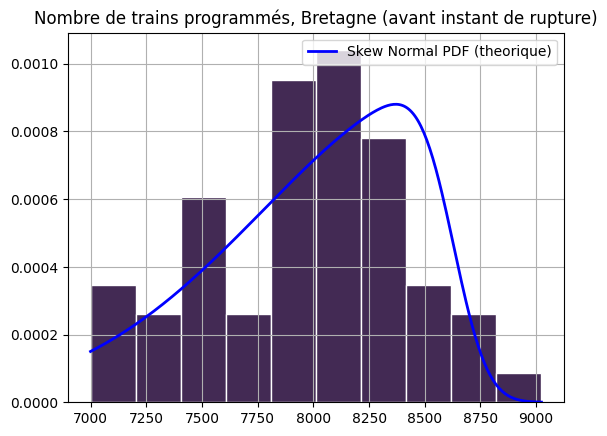
\includegraphics[width=0.7\textwidth]{image/BR-FIG5.png}
  \caption{Histogramme de l'échantillon avant point de rupture}
\end{figure}

\begin{figure}[H]
  \centering
  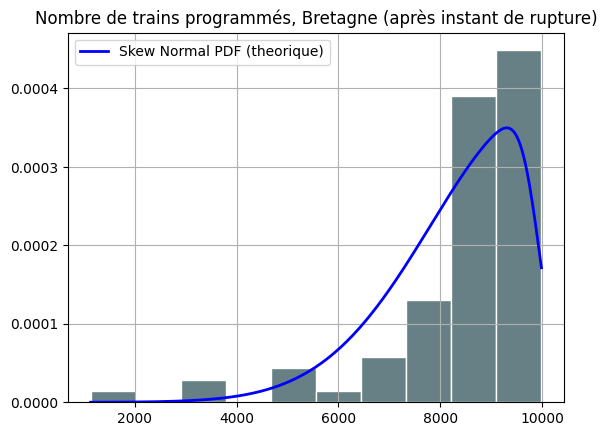
\includegraphics[width=0.7\textwidth]{image/BR-FIG6.png}
  \caption{Histogramme de l'échantillon après point de rupture}
\end{figure}

Nous avons obtenu un paramètre $\hat{\theta}^k$ négatif, indiquant des lois normales asymétriques inclinées vers la droite, ce qui signifie une queue de distribution plus longue du côté gauche. Cette caractéristique semble concorder avec les histogrammes présentés, où l'on observe une concentration plus importante des valeurs à gauche de la moyenne.

\subsection{Trains annulés}

\begin{figure}[H]
  \centering
  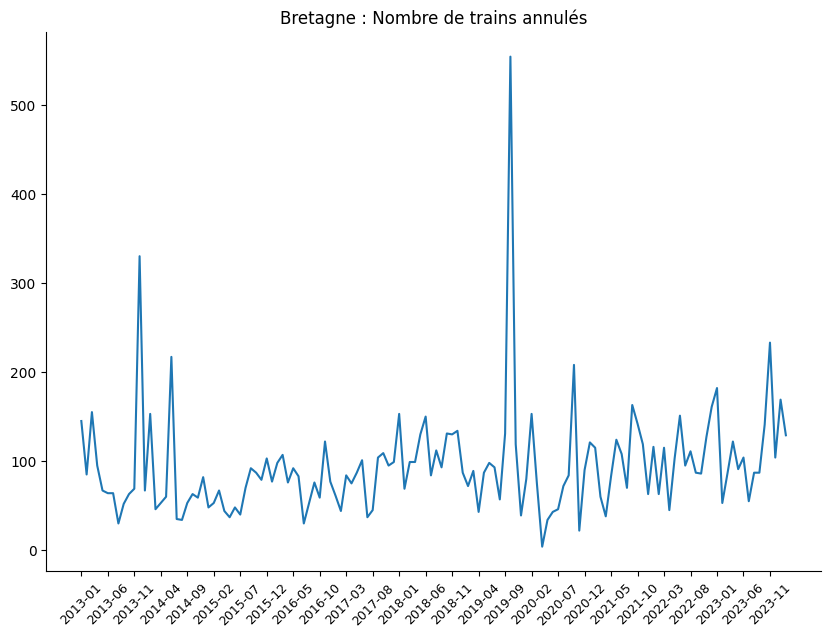
\includegraphics[width=0.7\textwidth]{image/BR-FIG07.png}
  \caption{Nombre de trains annulés entre 01/2013 et 02/2024}
\end{figure}

\begin{figure}[H]
  \centering
  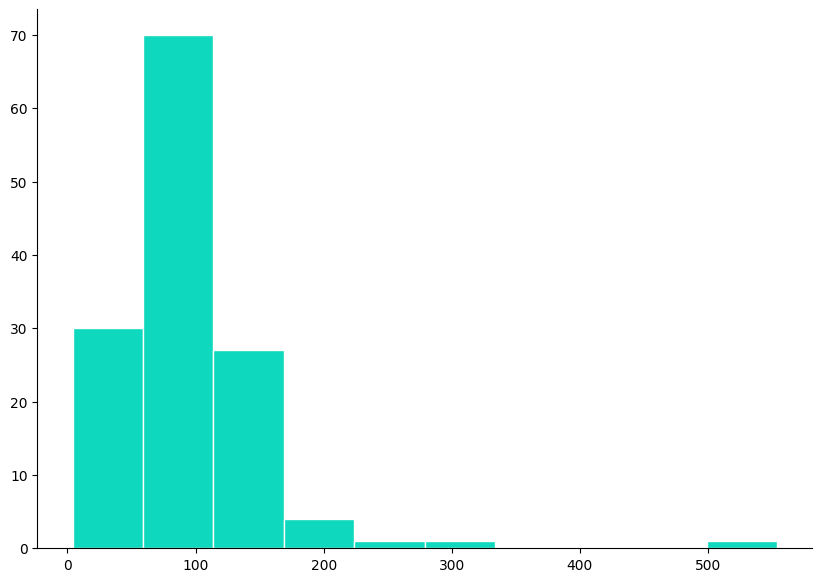
\includegraphics[width=0.7\textwidth]{image/BR-FOG08.png}
  \caption{Histogramme du nombre de trains annulés}
\end{figure}

Nous appliquons notre méthode de detection de point de rupture et nous obtenons les résultats suivants:

\subsubsection{Moment de rupture $\hat{k}$}

La date de rupture obtenue est: \textbf{2019-09}. 


\begin{figure}[H]
\centering
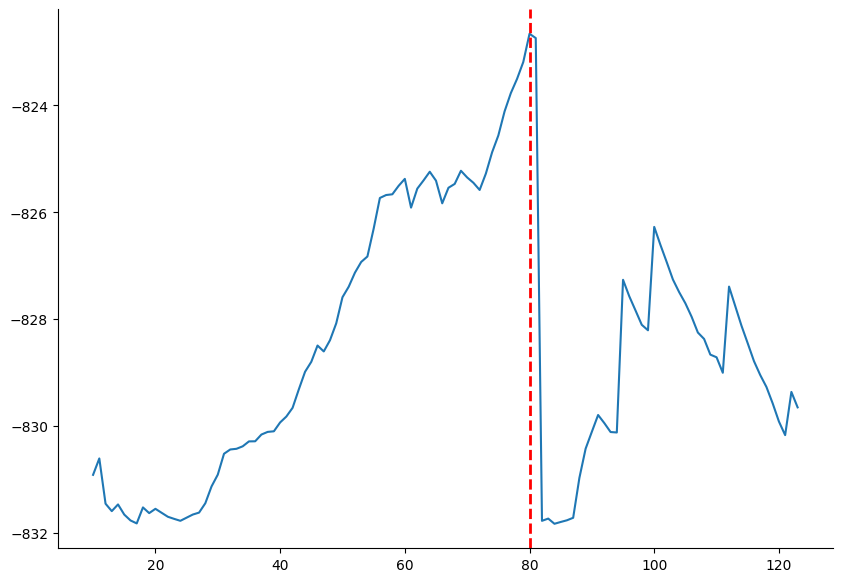
\includegraphics[width=0.8\textwidth]{image/BR-FIG10.png} 
\caption{Bretagne : Recherche du moment de rupture optimal.}
\label{fig:trains_ANNULES_2}
\end{figure}


\begin{figure}[H]
\centering
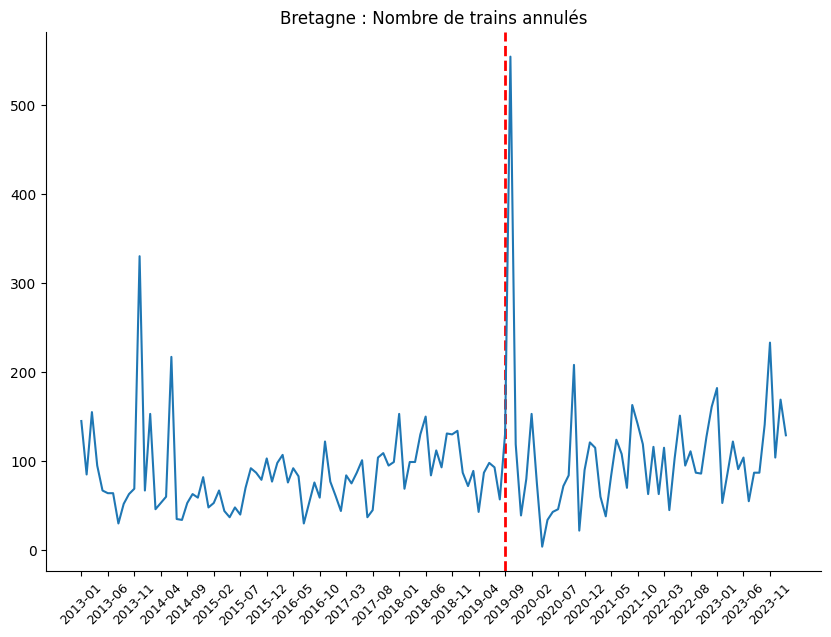
\includegraphics[width=0.8\textwidth]{image/BR-FIG09.png} 
\caption{Bretagne : La date de repture.}
\label{fig:trains_ANNULES_2}
\end{figure}




\subsubsection{Test de Kolmogorov-Smirnov}

Nous appliquons le test de Kolmogorov-Smirnov aux deux échantillons. Nous obtenons \textbf{p-value=  0.01}: nous rejettons $H_0$, ainsi le point de rupture est pertinent.

\subsubsection{Évaluation des paramètres des lois}

$\hat{\mu_1}^k$,$\hat{\mu_2}^k$,$\hat{\sigma_1}^k$,$\hat{\sigma_2}^k$,$\hat{\theta}^k$=( 35.10, 26.35, 66.08,  113.60, 7.86)\\

Nous constatons que la moyenne du nombre de trains annulés avant le point de rupture ($\hat{\mu_1}^k$) est supérieure à celle après le point de rupture ($\hat{\mu_2}^k$), ce qui indique une réduction du nombre moyen de trains annulés post-rupture. De plus, l'augmentation significative de la variance après le point de rupture ($\hat{\sigma_2}^k$ comparée à $\hat{\sigma_1}^k$) suggère une plus grande dispersion dans le nombre de trains annulés. Ces observations sont cohérentes avec les tendances visualisées dans la Figure 3.10.\\

Ci-dessous, nous comparons les histogrammes des deux échantillons aux lois théoriques (\textit{cf Figures 3.5 et 3.6})

\begin{figure}[H]
  \centering
  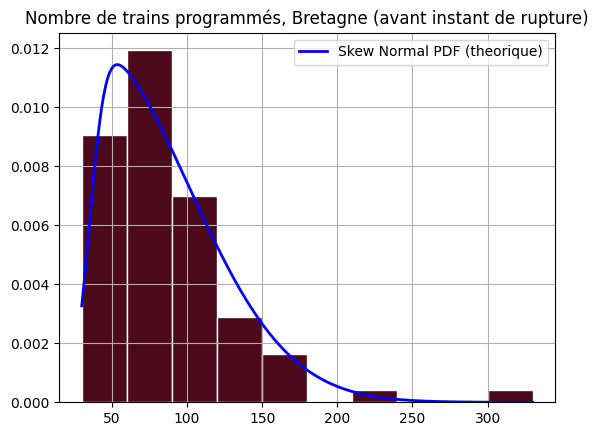
\includegraphics[width=0.7\textwidth]{image/BR-FIG11.png}
  \caption{Histogramme de l'échantillon avant point de rupture}
\end{figure}

\begin{figure}[H]
  \centering
  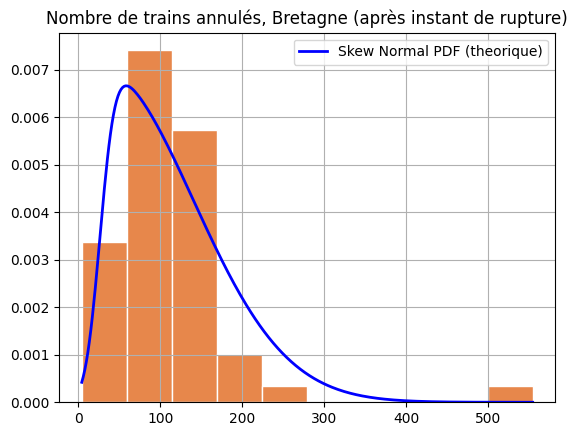
\includegraphics[width=0.7\textwidth]{image/BR-FIG12.png}
  \caption{Histogramme de l'échantillon après point de rupture}
\end{figure}


Nous avons obtenu un paramètre $\hat{\theta}^k$ positif, ce qui suggère des lois normales asymétriques avec une queue de distribution plus étendue vers la droite. Cette caractéristique est cohérente avec les histogrammes présentés pour l'échantillon avant et après le point de rupture. En effet, les histogrammes indiquent une asymétrie où la queue droite de la distribution s'étend au-delà de la moyenne plus que la queue gauche, conformément à une asymétrie positive.


\section{Pays-de-la-Loire}

\subsection{Trains programmés}

\begin{figure}[H]
\centering
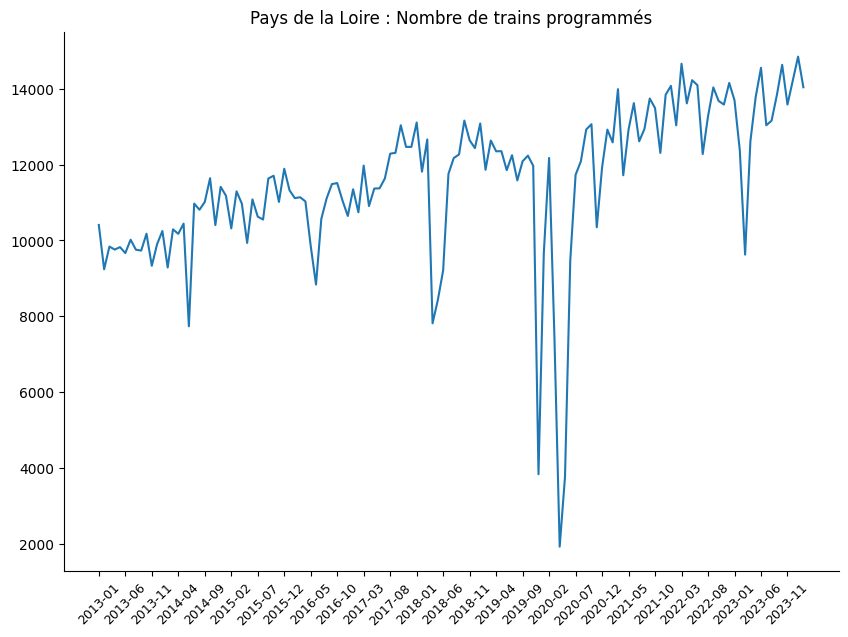
\includegraphics[width=0.8\textwidth]{image/PL-FIG01.png} 
\caption{Nombre de trains programmés de 2013 à 2024.}
\label{fig:trains_programmes}
\end{figure}

\begin{figure}[H]
\centering
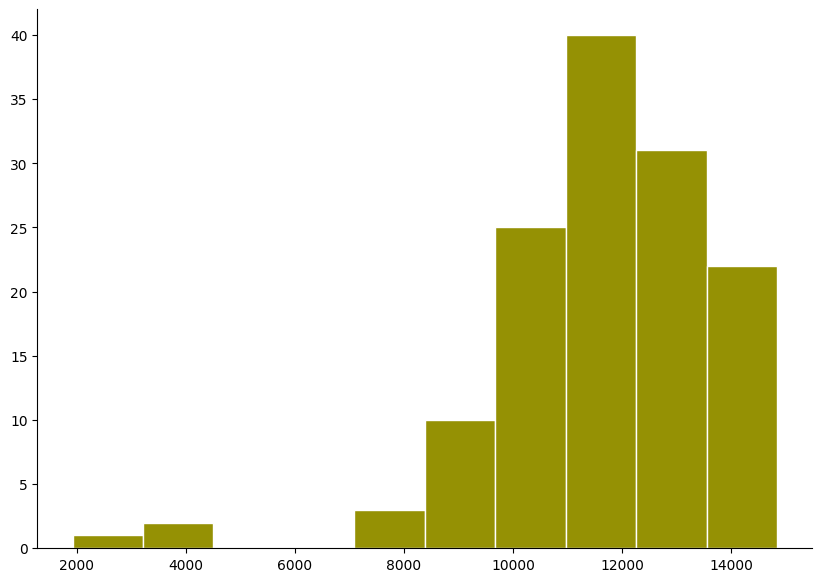
\includegraphics[width=0.8\textwidth]{image/PL-FIG02.png} 
\caption{Régions selectionnées.}
\label{fig:trains_programmes_2}
\end{figure}


Nous appliquons notre méthode de detection de point de rupture et nous obtenons les résultats suivants:

\subsubsection{Moment de rupture $\hat{k}$}

La date de rupture obtenue est: \textbf{2017-05}. 


\begin{figure}[H]
\centering
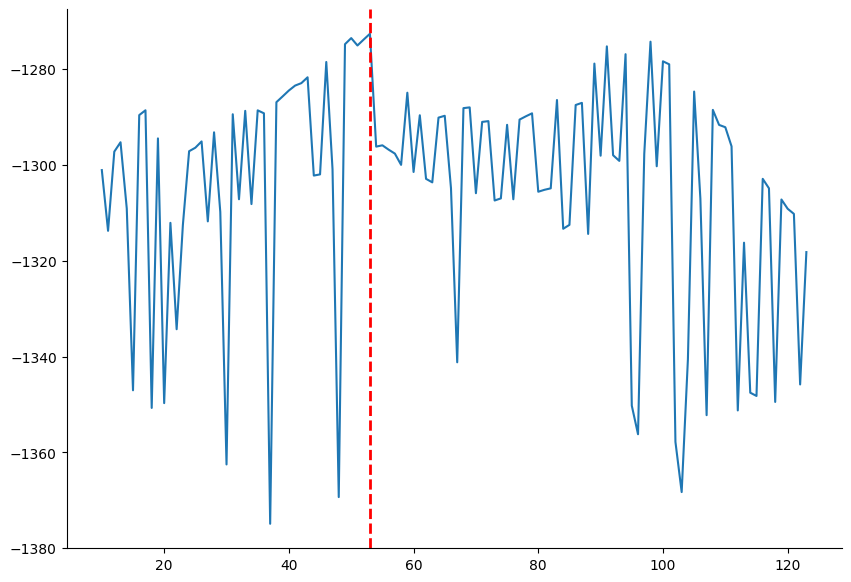
\includegraphics[width=0.75\textwidth]{image/PL-FIG03.png} 
\caption{Recherche du moment de rupture optimal.}
\label{fig:trains_ANNULES_2}
\end{figure}


\begin{figure}[H]
\centering
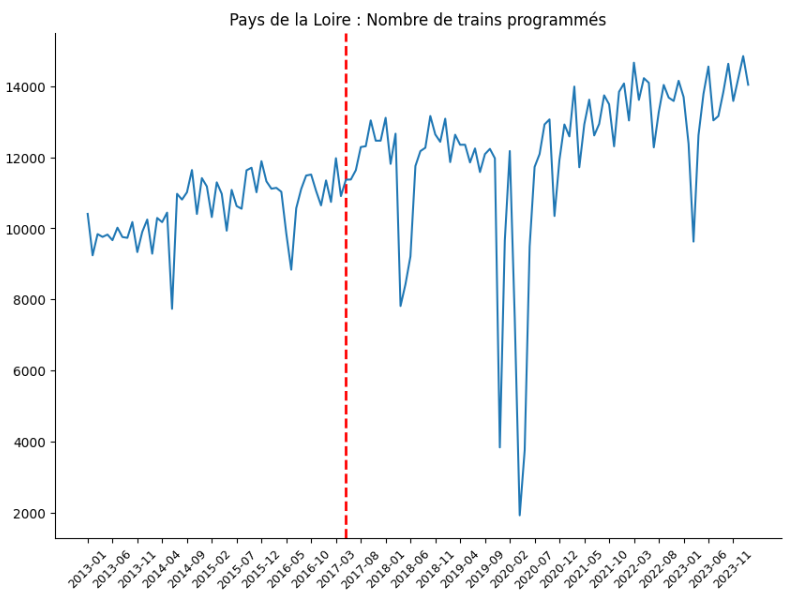
\includegraphics[width=0.8\textwidth]{Loire_rupt.png} 
\caption{La date de repture.}
\label{fig:trains_programmes_2}
\end{figure}

\subsubsection{Test de Kolmogorov-Smirnov}

Nous appliquons le test de Kolmogorov-Smirnov aux deux échantillons. Nous obtenons \textbf{p-value= 1.42e-20}: nous rejectons $H_0$.

\subsubsection{Évaluation des paramètres des lois}

$\hat{\mu_1}^k$,$\hat{\mu_2}^k$,$\hat{\sigma_1}^k$,$\hat{\sigma_2}^k$,$\hat{\theta}^k$=( 11737.96, 14503.91, 1459.96, 3231.32,-7.89)\\
 
Nous observons que la moyenne du nombre de trains programmés dans les Pays de la Loire avant le point de rupture ($\hat{\mu_1}^k$) est moins élevée que celle après le point de rupture ($\hat{\mu_2}^k$), révélant une augmentation notable du nombre moyen de trains programmés après la rupture. Parallèlement, la variance après le point de rupture ($\hat{\sigma_2}^k$) dépasse significativement celle d'avant la rupture ($\hat{\sigma_1}^k$), ce qui indique une plus grande hétérogénéité dans la programmation des trains suite à cette date. 


Ci-dessous, nous comparons les histogrammes des deux échantillons aux lois théoriques (\textit{cf Figures 3.17 et 3.18})

\begin{figure}[H]
  \centering
  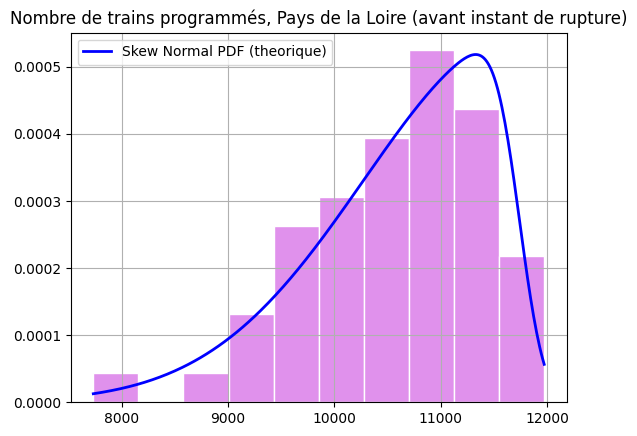
\includegraphics[width=0.7\textwidth]{image/PL-FIG04.png}
  \caption{Histogramme de l'échantillon avant point de rupture}
\end{figure}

\begin{figure}[H]
  \centering
  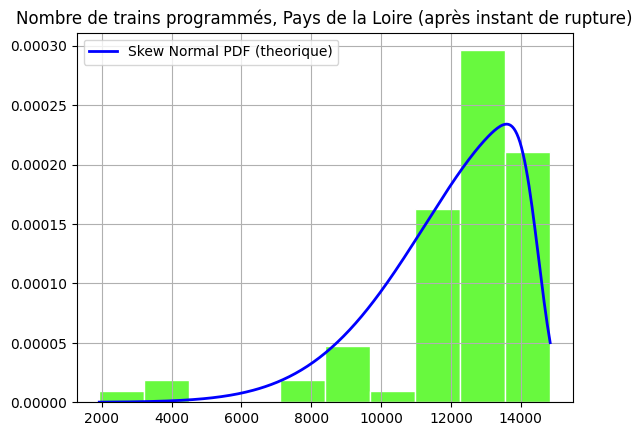
\includegraphics[width=0.7\textwidth]{image/PL-FIG05.png}
  \caption{Histogramme de l'échantillon après point de rupture}
\end{figure}

Nous avons obtenu un paramètre $\hat{\theta}^k$ négatif, suggérant des distributions normales asymétriques inclinées vers la droite, impliquant ainsi une queue de distribution plus longue du côté gauche. Cette asymétrie est validée par les histogrammes présentés, où l'on constate une concentration accrue des valeurs à droite de la moyenne, spécialement dans les données après le point de rupture. Cette tendance indique que dans les Pays de la Loire, les trains programmés tendent à présenter une distribution avec une incidence plus marquée de valeurs extrêmement élevées suite au point de rupture, comme le montrent les Figures 3.17 et 3.18.


\subsection{Trains annulés}

\begin{figure}[H]
  \centering
  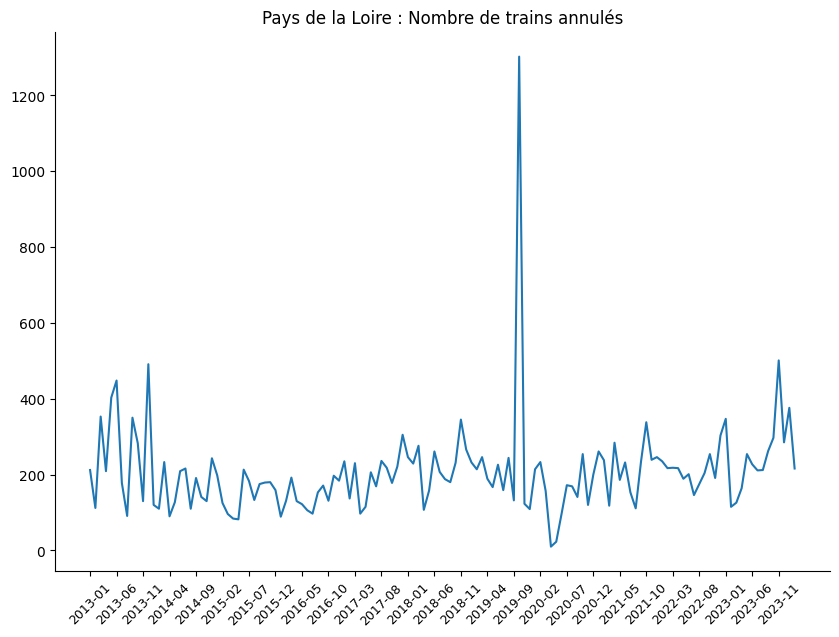
\includegraphics[width=0.7\textwidth]{image/PL-FIG06.png}
  \caption{Nombre de trains annulés entre 01/2013 et 02/2024}
\end{figure}

\begin{figure}[H]
  \centering
  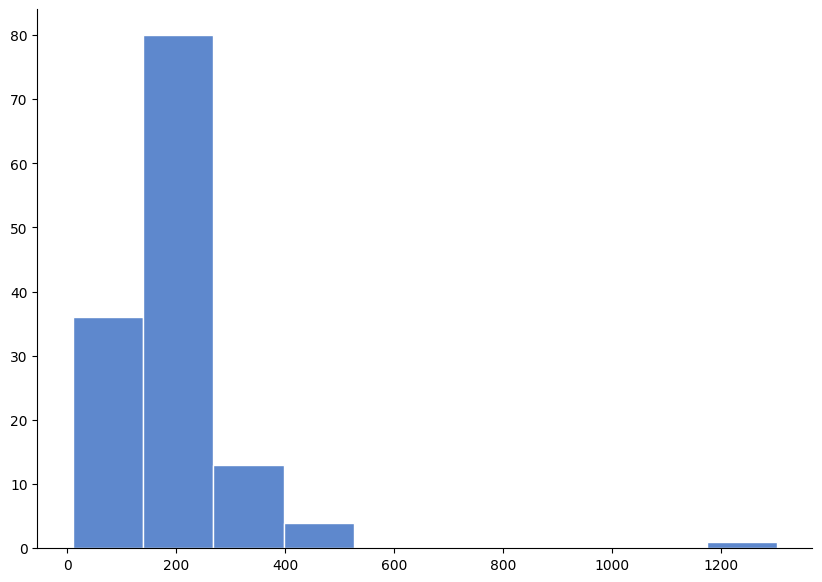
\includegraphics[width=0.7\textwidth]{image/PL-FIG07.png}
  \caption{Histogramme du nombre de trains annulés}
\end{figure}

Nous appliquons notre méthode de detection de point de rupture et nous obtenons les résultats suivants:

\subsubsection{Moment de rupture $\hat{k}$}

La date de rupture obtenue est: \textbf{2019-09}. 


\begin{figure}[H]
\centering
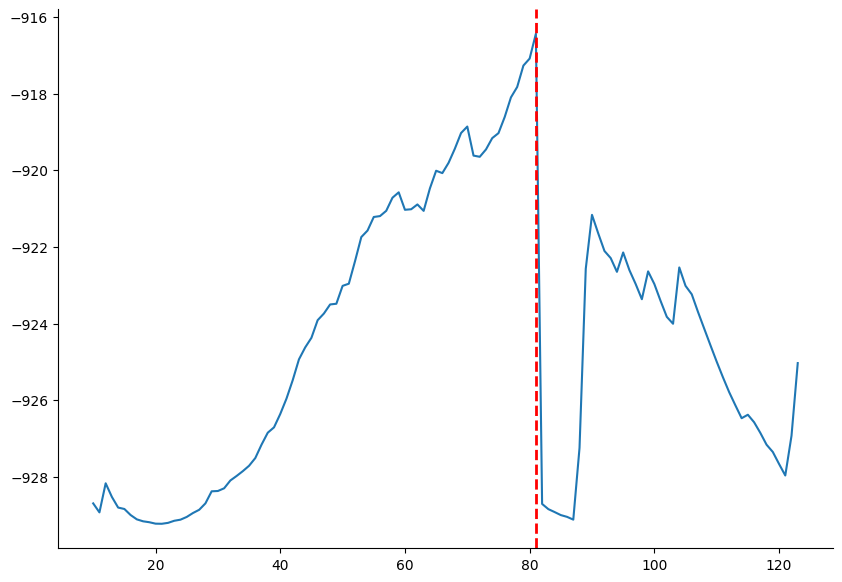
\includegraphics[width=0.8\textwidth]{image/PL-FIG08.png} 
\caption{Recherche du moment de rupture optimal.}
\label{fig:trains_ANNULES_2}
\end{figure}


\begin{figure}[H]
\centering
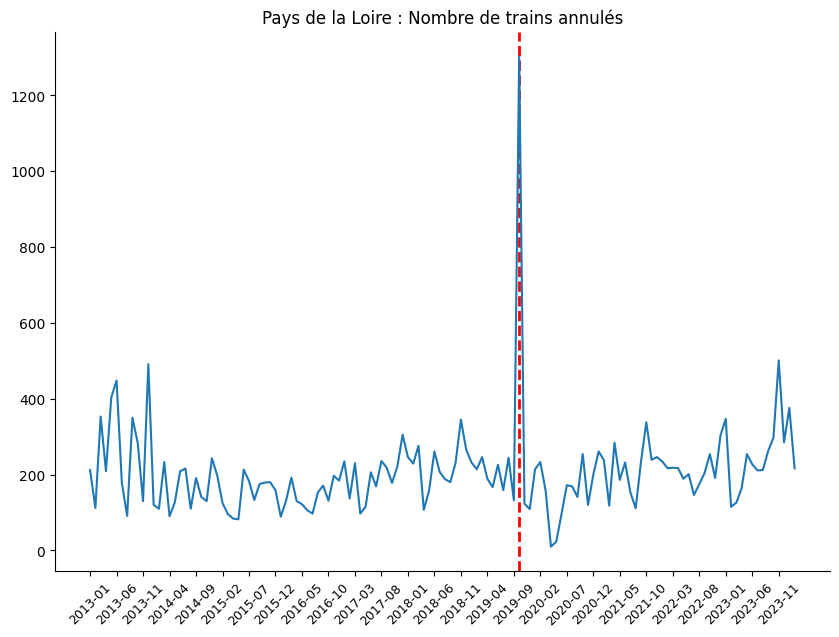
\includegraphics[width=0.8\textwidth]{image/PL-FIG09.png} 
\caption{La date de repture.}
\label{fig:trains_ANNULES_2}
\end{figure}




\subsubsection{Test de Kolmogorov-Smirnov}

Nous appliquons le test de Kolmogorov-Smirnov aux deux échantillons. Nous obtenons \textbf{p-value= 0.17 }: nous ne pouvons pas rejeter $H_0$. Le point de rupture ne semble pas pertinent.

\subsubsection{Évaluation des paramètres des lois}

$\hat{\mu_1}^k$,$\hat{\mu_2}^k$,$\hat{\sigma_1}^k$,$\hat{\sigma_2}^k$,$\hat{\theta}^k$=( 92.92,  68.23, 125.48, 239.38, 6.28)\\

Nous constatons que la moyenne du nombre de trains annulés dans les Pays de la Loire avant le point de rupture ($\hat{\mu_1}^k$) est plus élevée que celle après le point de rupture ($\hat{\mu_2}^k$), révélant ainsi une diminution du nombre moyen de trains annulés suite à la rupture. En outre, l'augmentation de la variance post-rupture ($\hat{\sigma_2}^k$ par rapport à $\hat{\sigma_1}^k$) indique une variabilité plus importante dans le nombre de trains annulés après le point de rupture. Le paramètre de skewness positif ($\hat{\theta}^k$) suggère une distribution asymétrique avec une queue plus prononcée vers la droite. Cette distribution est visuellement corroborée par la Figure 3.22, qui montre un changement significatif dans la distribution des annulations de trains à la date indiquée par le trait rouge en pointillé.\\

Ci-dessous, nous comparons les histogrammes des deux échantillons aux lois théoriques (\textit{cf Figures 3.23 et 3.24})

\begin{figure}[H]
  \centering
  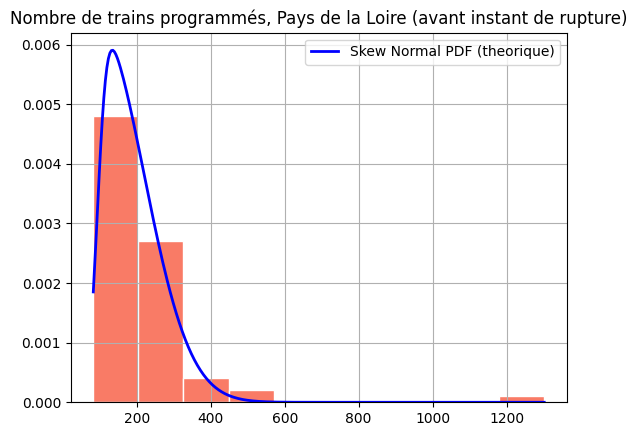
\includegraphics[width=0.7\textwidth]{image/PL-FIG10.png}
  \caption{Histogramme de l'échantillon avant point de rupture}
\end{figure}

\begin{figure}[H]
  \centering
  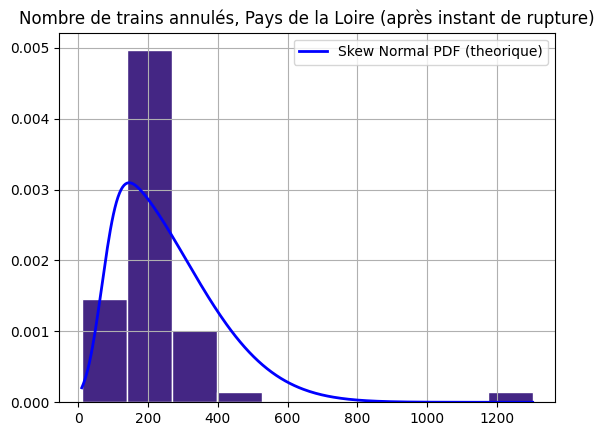
\includegraphics[width=0.7\textwidth]{image/PL-FIG11.png}
  \caption{Histogramme de l'échantillon après point de rupture}
\end{figure}

Nous avons obtenu un paramètre $\hat{\theta}^k$ positif, indiquant des distributions normales asymétriques avec une queue plus longue s'étendant vers la droite. Cette caractéristique se vérifie dans les histogrammes pour l'échantillon avant et après le point de rupture, où l'on constate une concentration des valeurs dépassant la moyenne sur le côté droit de la distribution. 

\section{Centre}

\subsection{Trains programmés}

\begin{figure}[H]
\centering
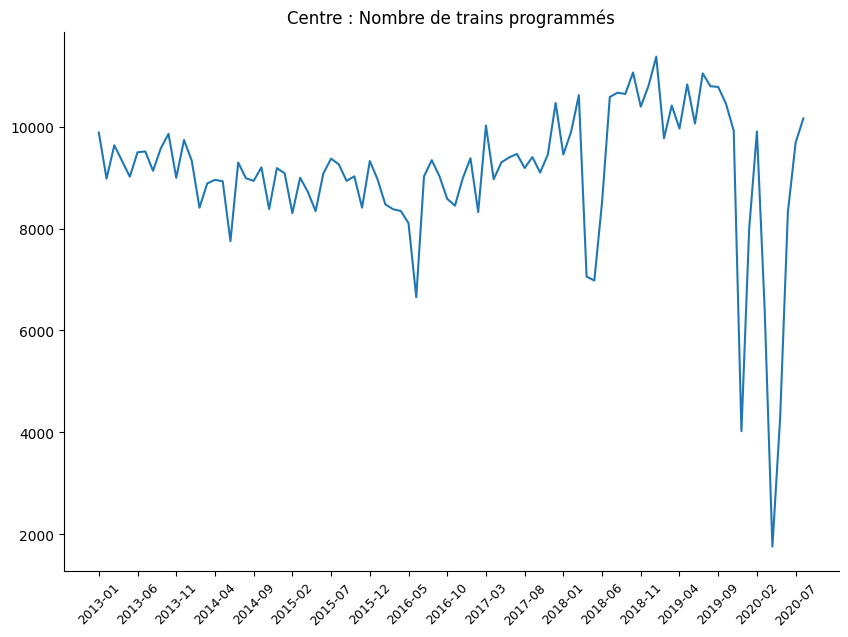
\includegraphics[width=0.8\textwidth]{image/Cn-FIG1.png} 
\caption{Nombre de trains programmés de 2013 à 2024.}
\label{fig:trains_programmes}
\end{figure}

\begin{figure}[H]
\centering
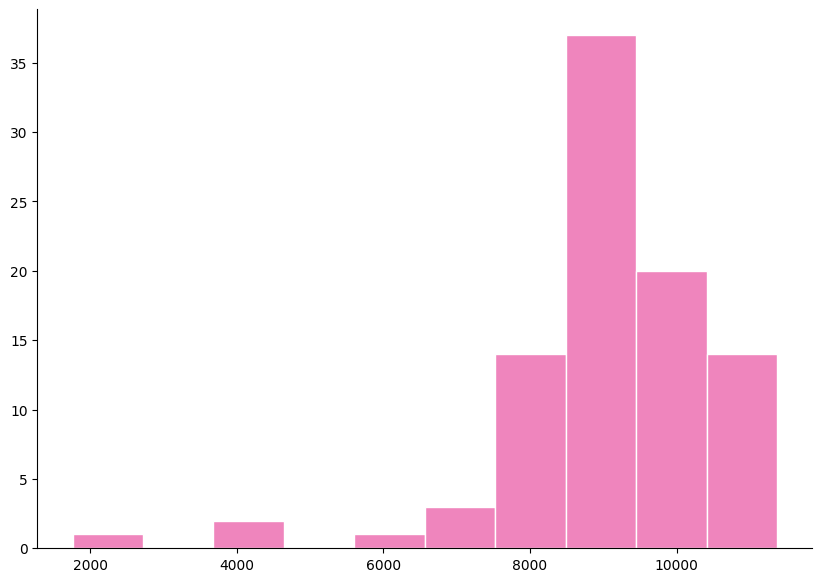
\includegraphics[width=0.8\textwidth]{image/Cn-FIG02.png} 
\caption{Régions selectionnées.}
\label{fig:trains_programmes_2}
\end{figure}


Nous appliquons notre méthode de detection de point de rupture et nous obtenons les résultats suivants:

\subsubsection{Moment de rupture $\hat{k}$}

La date de rupture obtenue est: \textbf{2017-10}. 


\begin{figure}[H]
\centering
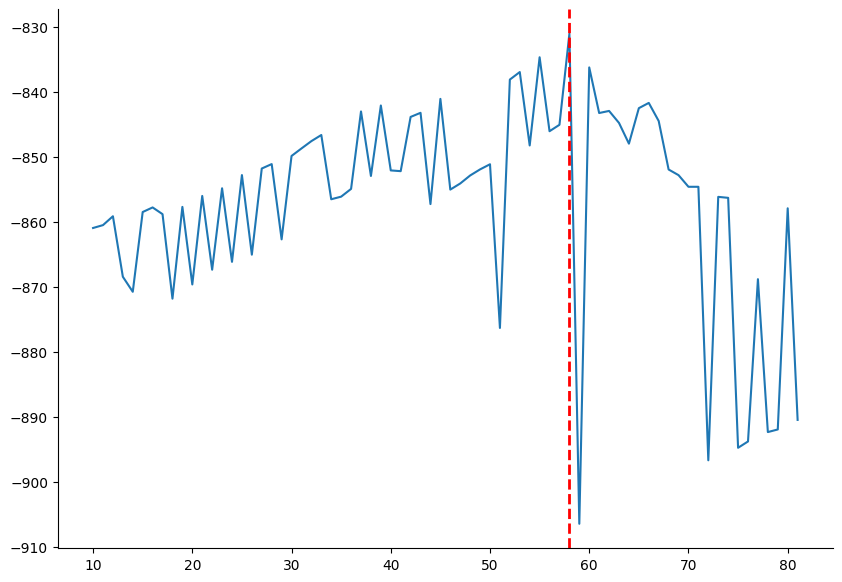
\includegraphics[width=0.75\textwidth]{image/Cn-FIG03.png} 
\caption{Recherche du moment de rupture optimal.}
\label{fig:trains_ANNULES_2}
\end{figure}


\begin{figure}[H]
\centering
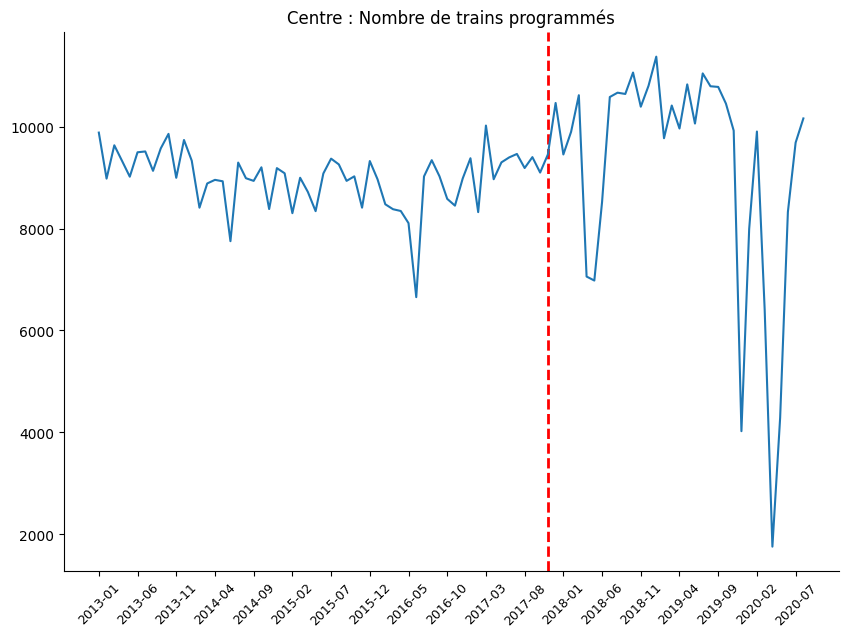
\includegraphics[width=0.8\textwidth]{Cn-FIG04.png} 
\caption{La date de repture.}
\label{fig:trains_programmes_2}
\end{figure}

\subsubsection{Test de Kolmogorov-Smirnov}

Nous appliquons le test de Kolmogorov-Smirnov aux deux échantillons. Nous obtenons \textbf{p-value=  4.651e-08}: nous rejectons $H_0$.

\subsubsection{Évaluation des paramètres des lois}

$\hat{\mu_1}^k$,$\hat{\mu_2}^k$,$\hat{\sigma_1}^k$,$\hat{\sigma_2}^k$,$\hat{\theta}^k$=(9.68897541e+03  1.13077069e+04  9.30181789e+02  2.86048081e+03
 -4.93819171e+00)\\
 
Nous observons que la moyenne du nombre de trains programmés dans la région Centre avant le point de rupture ($\hat{\mu_1}^k$) est inférieure à celle après le point de rupture ($\hat{\mu_2}^k$), suggérant une augmentation significative du nombre moyen de trains programmés post-rupture. De même, la variance post-rupture ($\hat{\sigma_2}^k$) est nettement plus élevée que la variance pré-rupture ($\hat{\sigma_1}^k$), indiquant une diversité accrue dans le nombre de trains programmés après cette date. Le skewness négatif ($\hat{\theta}^k$) reflète une asymétrie de la distribution, avec une tendance à des valeurs extrêmement basses plus fréquentes. Ces observations sont cohérentes avec le changement marqué illustré dans la Figure 3.28, où la ligne rouge en pointillé indique le moment de la rupture.

Ci-dessous, nous comparons les histogrammes des deux échantillons aux lois théoriques (\textit{cf Figures 3.29 et 3.30})

\begin{figure}[H]
  \centering
  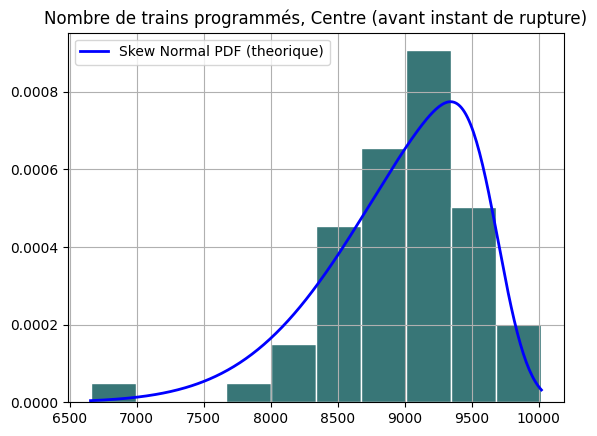
\includegraphics[width=0.7\textwidth]{image/Cn-FIG05.png}
  \caption{Histogramme de l'échantillon avant point de rupture}
\end{figure}

\begin{figure}[H]
  \centering
  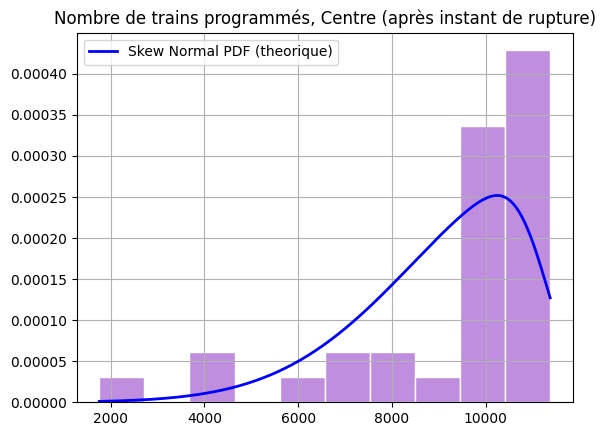
\includegraphics[width=0.7\textwidth]{image/Cn-FIG06.png}
  \caption{Histogramme de l'échantillon après point de rupture}
\end{figure}

Nous avons obtenu un paramètre $\hat{\theta}^k$ négatif, ce qui indique des distributions normales asymétriques inclinées vers la gauche, résultant en une queue de distribution allongée du côté droit. Cette asymétrie se vérifie dans les histogrammes, où nous observons une augmentation des valeurs supérieures à la moyenne, en particulier après le point de rupture. Cette observation suggère que dans la région Centre, la distribution des trains programmés post-rupture est marquée par une fréquence accrue de valeurs élevées, comme l'illustrent les Figures 3.29 et 3.30.

\subsection{Trains annulés}

\begin{figure}[H]
  \centering
  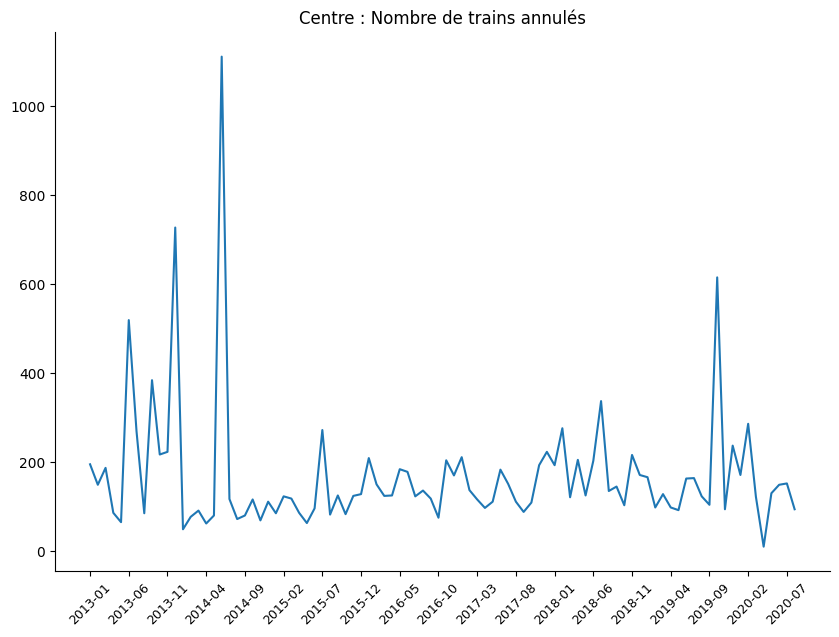
\includegraphics[width=0.7\textwidth]{image/Cn-FIG07.png}
  \caption{Nombre de trains annulés entre 01/2013 et 02/2024}
\end{figure}

\begin{figure}[H]
  \centering
  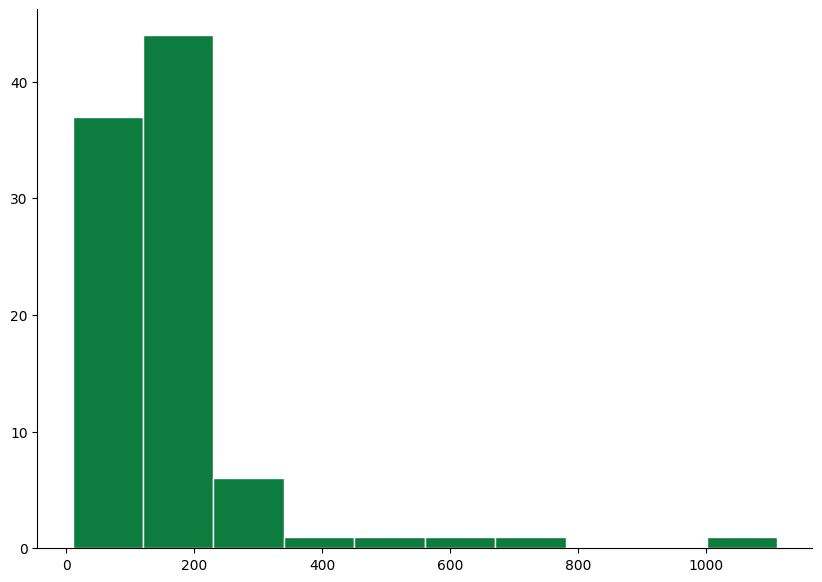
\includegraphics[width=0.7\textwidth]{image/Cn-FIG08.png}
  \caption{Histogramme du nombre de trains annulés}
\end{figure}

Nous appliquons notre méthode de detection de point de rupture et nous obtenons les résultats suivants:

\subsubsection{Moment de rupture $\hat{k}$}

La date de rupture obtenue est: \textbf{2014-06}. 


\begin{figure}[H]
\centering
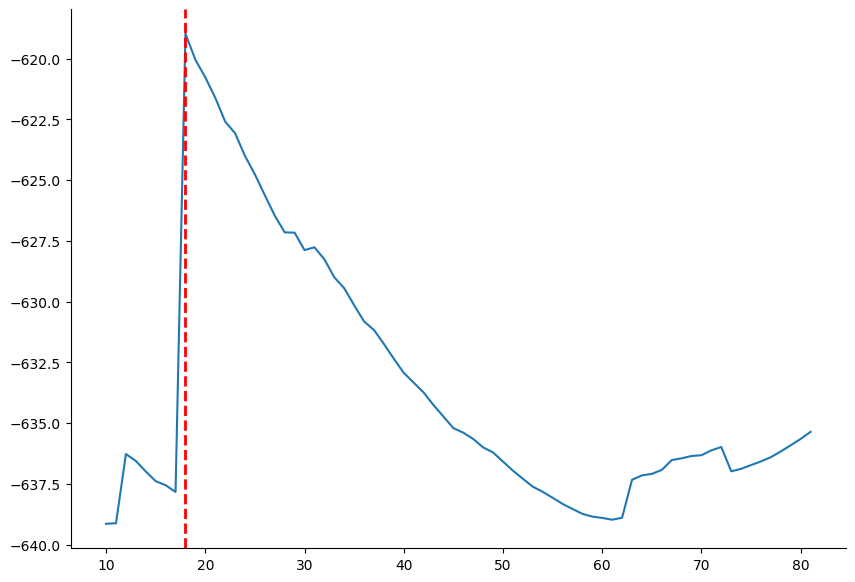
\includegraphics[width=0.8\textwidth]{image/Cn-FIG09.png} 
\caption{Recherche du moment de rupture optimal.}
\label{fig:trains_ANNULES_2}
\end{figure}


\begin{figure}[H]
\centering
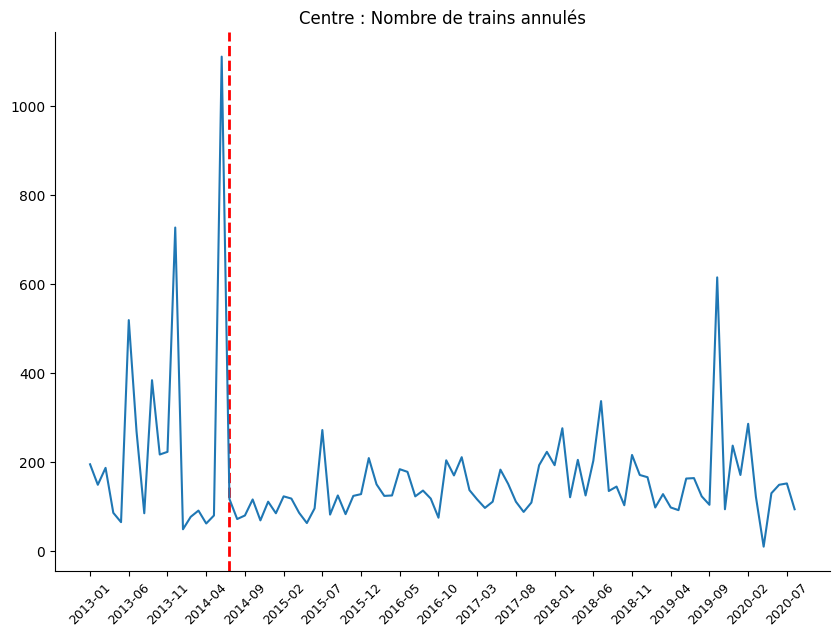
\includegraphics[width=0.8\textwidth]{image/Cn-FIG10.png} 
\caption{La date de repture.}
\label{fig:trains_ANNULES_2}
\end{figure}


\subsubsection{Test de Kolmogorov-Smirnov}

Nous appliquons le test de Kolmogorov-Smirnov aux deux échantillons. Nous obtenons \textbf{p-value= 0.17 }: nous ne pouvons pas rejeter $H_0$. Le point de rupture ne semble pas pertinent.

\subsubsection{Évaluation des paramètres des lois}


$\hat{\mu_1}^k$,$\hat{\mu_2}^k$,$\hat{\sigma_1}^k$,$\hat{\sigma_2}^k$,$\hat{\theta}^k$=(  9.66, 66.37, 343.50, 114.80, 5.30)\\

Nous observons que la moyenne du nombre de trains annulés dans la région Centre avant le point de rupture ($\hat{\mu_1}^k$) est inférieure à celle observée après le point de rupture ($\hat{\mu_2}^k$), suggérant une augmentation du nombre moyen de trains annulés suite à la rupture. De plus, l'accroissement de la variance après le point de rupture ($\hat{\sigma_2}^k$ comparativement à $\hat{\sigma_1}^k$) indique une plus grande dispersion dans le nombre de trains annulés post-rupture. Le paramètre de skewness positif ($\hat{\theta}^k$) révèle une asymétrie de la distribution, avec une queue s'étendant davantage vers la droite. Cette asymétrie est confirmée visuellement par la Figure 3.34, où le changement notable dans la distribution des annulations de trains est mis en évidence par la ligne rouge en pointillé indiquant le moment de la rupture.


Ci-dessous, nous comparons les histogrammes des deux échantillons aux lois théoriques (\textit{cf Figures 3.35 et 3.36})

\begin{figure}[H]
  \centering
  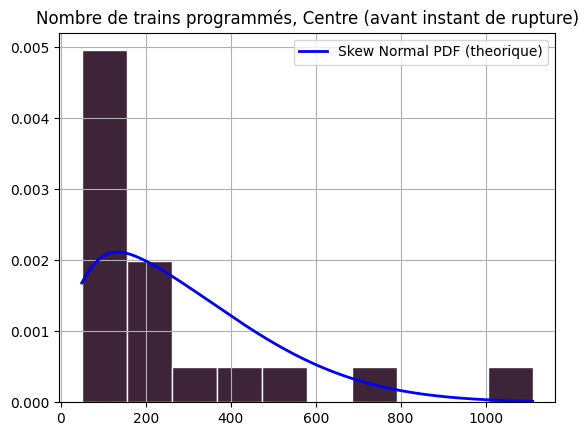
\includegraphics[width=0.7\textwidth]{image/Cn-FIG11.png}
  \caption{Histogramme de l'échantillon avant point de rupture}
\end{figure}

\begin{figure}[H]
  \centering
  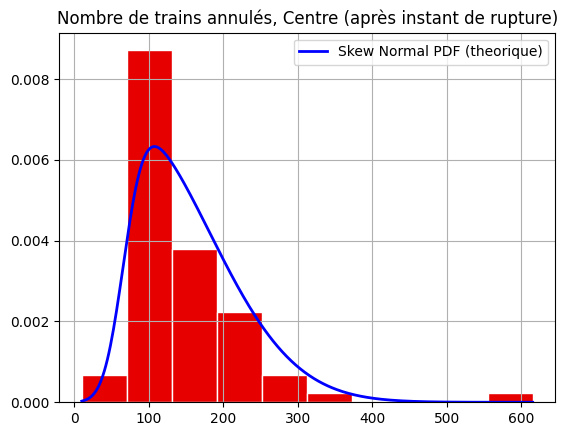
\includegraphics[width=0.7\textwidth]{image/Cn-FIG12.png}
  \caption{Histogramme de l'échantillon après point de rupture}
\end{figure}

Nous avons obtenu un paramètre $\hat{\theta}^k$ positif, indiquant des distributions normales asymétriques avec une queue de distribution s’étendant plus longuement vers la droite. Cette caractéristique est confirmée par les histogrammes de la région Centre, tant pour l'échantillon avant qu'après le point de rupture. Les données montrent une prédominance des valeurs excédant la moyenne du côté droit, ce qui est caractéristique d'une skewness positive. Cette asymétrie dans la distribution du nombre de trains annulés est illustrée visuellement par les Figures 3.35 et 3.36, soulignant la présence d'une distribution inclinée post-rupture dans la région étudiée.


\section{Aquitaine}

\subsection{Trains programmés}

\begin{figure}[H]
\centering
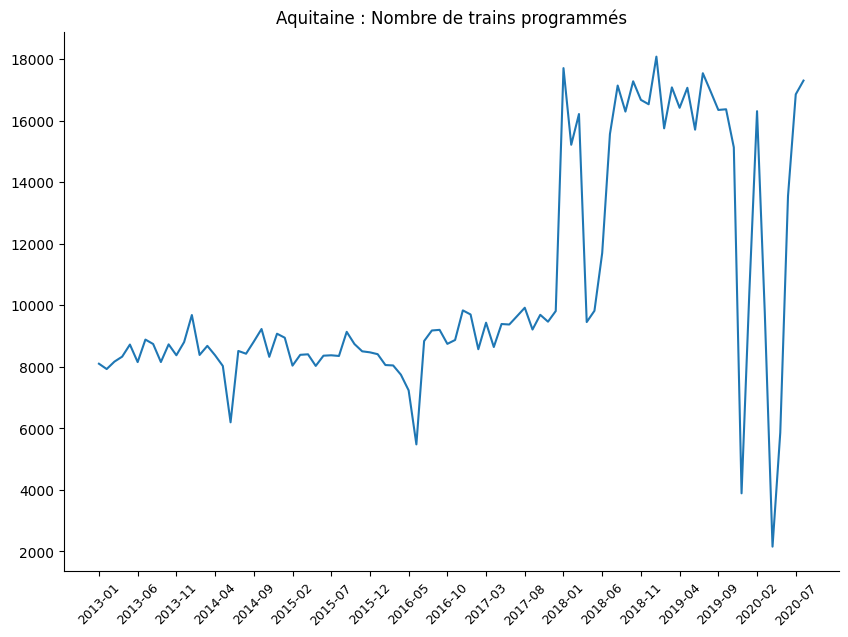
\includegraphics[width=0.8\textwidth]{image/AQ-FIG1.png} 
\caption{Nombre de trains programmés de 2013 à 2024.}
\label{fig:trains_programmes}
\end{figure}

\begin{figure}[H]
\centering
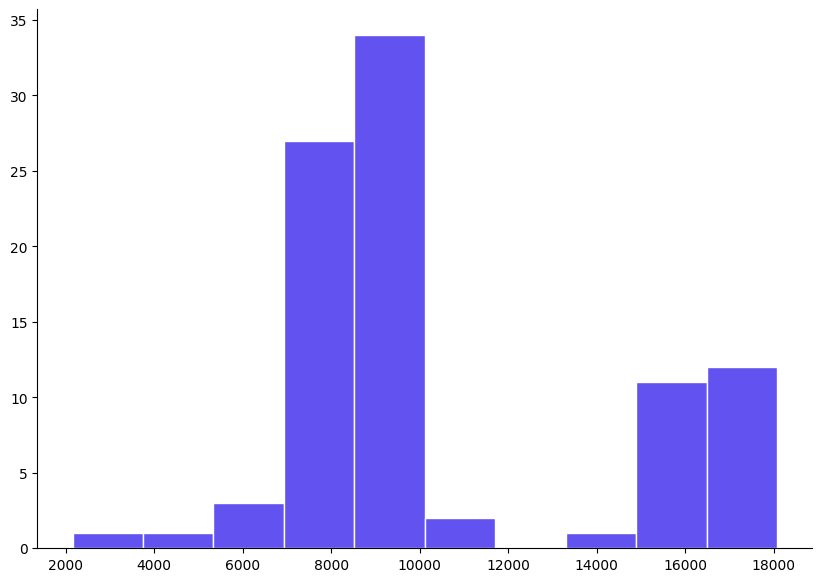
\includegraphics[width=0.8\textwidth]{image/AQ-FIG2.png} 
\caption{Régions selectionnées.}
\label{fig:trains_programmes_2}
\end{figure}


Nous appliquons notre méthode de detection de point de rupture et nous obtenons les résultats suivants:

\subsubsection{Moment de rupture $\hat{k}$}

La date de rupture obtenue est: \textbf{2017-11}. 


\begin{figure}[H]
\centering
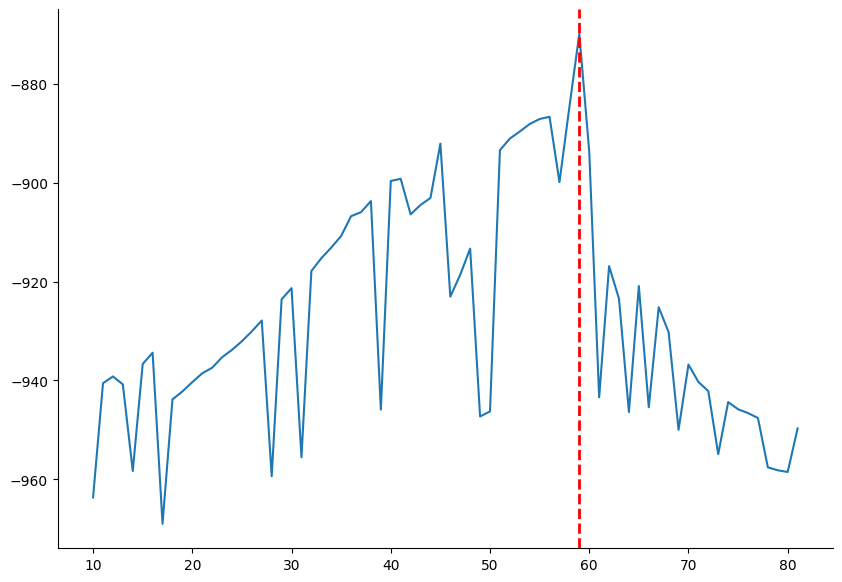
\includegraphics[width=0.75\textwidth]{image/AQ-FIG3.png} 
\caption{Recherche du moment de rupture optimal.}
\label{fig:trains_ANNULES_2}
\end{figure}


\begin{figure}[H]
\centering
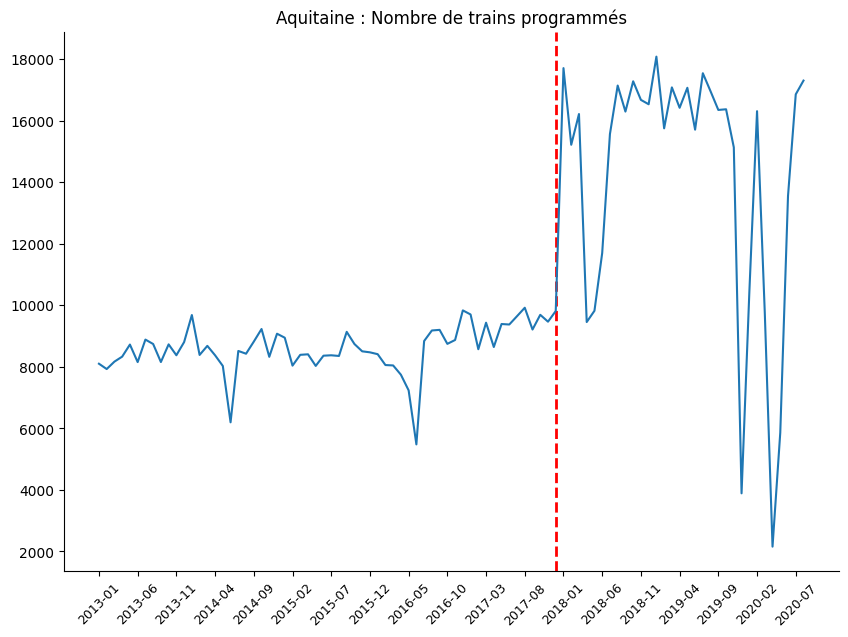
\includegraphics[width=0.8\textwidth]{image/AQ-FIG4.png} 
\caption{La date de repture.}
\label{fig:trains_programmes_2}
\end{figure}

\subsubsection{Test de Kolmogorov-Smirnov}

Nous appliquons le test de Kolmogorov-Smirnov aux deux échantillons. Nous obtenons \textbf{p-value=  1.5789521915581405e-15}: nous rejectons $H_0$.

\subsubsection{Évaluation des paramètres des lois}

$\hat{\mu_1}^k$,$\hat{\mu_2}^k$,$\hat{\sigma_1}^k$,$\hat{\sigma_2}^k$,$\hat{\theta}^k$=(9.79476421e+03  1.80417857e+04  1.43618833e+03  5.57450614e+03
 -1.31829067e+01)\\
 

Pour votre figure de la région Aquitaine et les valeurs des paramètres statistiques données, voici le paragraphe corrigé :

Nous observons que la moyenne du nombre de trains programmés dans la région Aquitaine avant le point de rupture ($\hat{\mu_1}^k$) est considérablement inférieure à celle qui est relevée après le point de rupture ($\hat{\mu_2}^k$), indiquant ainsi une augmentation marquée du nombre moyen de trains programmés post-rupture. En outre, nous notons que la variance après le point de rupture ($\hat{\sigma_2}^k$) surpasse largement celle d'avant la rupture ($\hat{\sigma_1}^k$), ce qui signale une variabilité beaucoup plus grande dans la fréquence des trains programmés suite à cette date. Le skewness négatif très prononcé ($\hat{\theta}^k$) suggère une asymétrie de la distribution, avec une prédominance de valeurs extrêmement basses. Ces observations sont illustrées par la Figure 3.40, où la ligne rouge en pointillé marque le point de rupture significatif dans la distribution du nombre de trains programmés.

Ci-dessous, nous comparons les histogrammes des deux échantillons aux lois théoriques (\textit{cf Figures 3.29 et 3.30})

\begin{figure}[H]
  \centering
  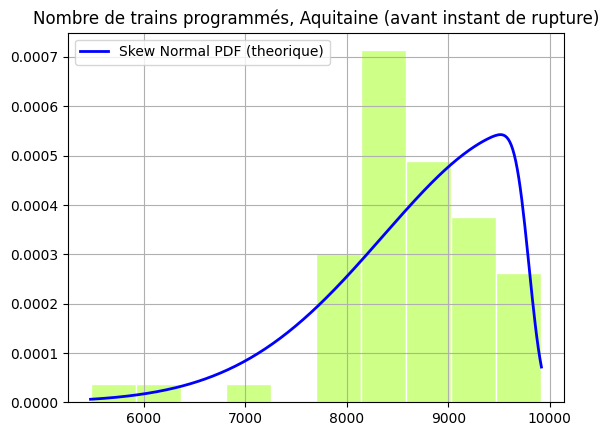
\includegraphics[width=0.7\textwidth]{image/AQ-FIG5.png}
  \caption{Histogramme de l'échantillon avant point de rupture}
\end{figure}

\begin{figure}[H]
  \centering
  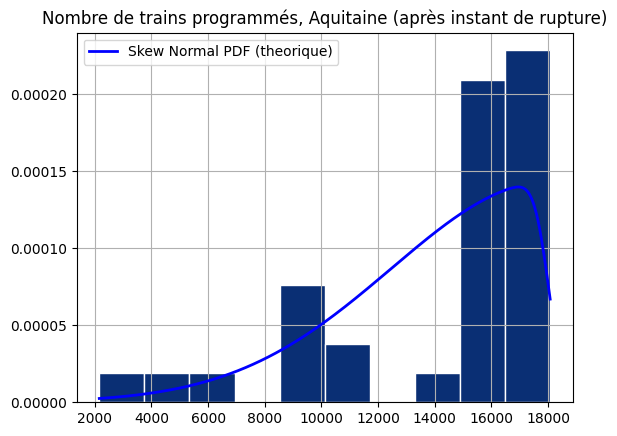
\includegraphics[width=0.7\textwidth]{image/AQ-FIG6.png}
  \caption{Histogramme de l'échantillon après point de rupture}
\end{figure}

Nous avons obtenu un paramètre $\hat{\theta}^k$ négatif, indiquant des distributions normales asymétriques inclinées vers la gauche, ce qui se traduit par une queue de distribution prolongée du côté droit. Cette asymétrie est confirmée par les histogrammes de la région Aquitaine, qui montrent un nombre accru de valeurs excédant la moyenne, surtout après le point de rupture. Cela indique que la distribution des trains programmés dans la région Aquitaine après le point de rupture tend vers une fréquence plus élevée de valeurs supérieures, comme démontré par les Figures 3.41 et 3.42, illustrant le changement dans la distribution post-rupture.

\subsection{Trains annulés}

\begin{figure}[H]
  \centering
  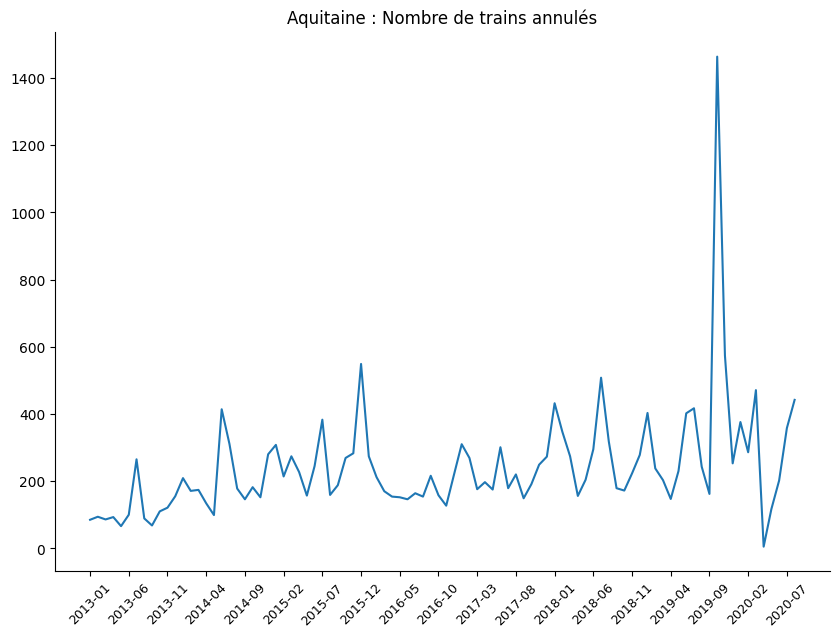
\includegraphics[width=0.7\textwidth]{image/AQ-FIG7.png}
  \caption{Nombre de trains annulés entre 01/2013 et 02/2024}
\end{figure}

\begin{figure}[H]
  \centering
  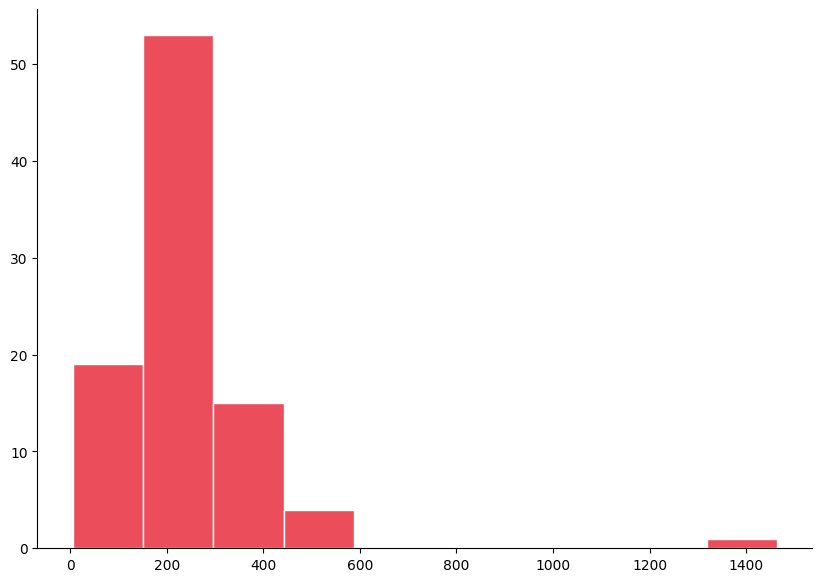
\includegraphics[width=0.7\textwidth]{image/AQ-FIG8.png}
  \caption{Histogramme du nombre de trains annulés}
\end{figure}

Nous appliquons notre méthode de detection de point de rupture et nous obtenons les résultats suivants:

\subsubsection{Moment de rupture $\hat{k}$}

La date de rupture obtenue est: \textbf{2019-10}. 


\begin{figure}[H]
\centering
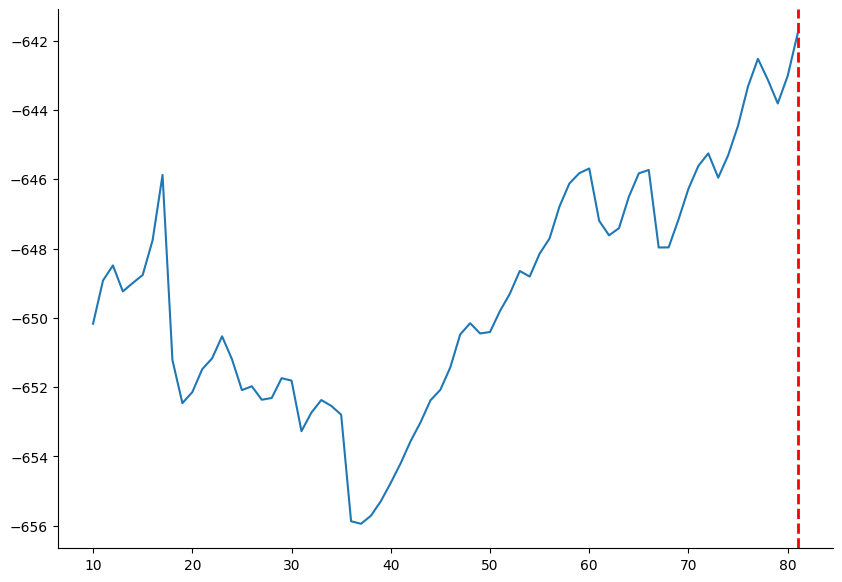
\includegraphics[width=0.8\textwidth]{image/AQ-FIG9.png} 
\caption{Recherche du moment de rupture optimal.}
\label{fig:trains_ANNULES_2}
\end{figure}


\begin{figure}[H]
\centering
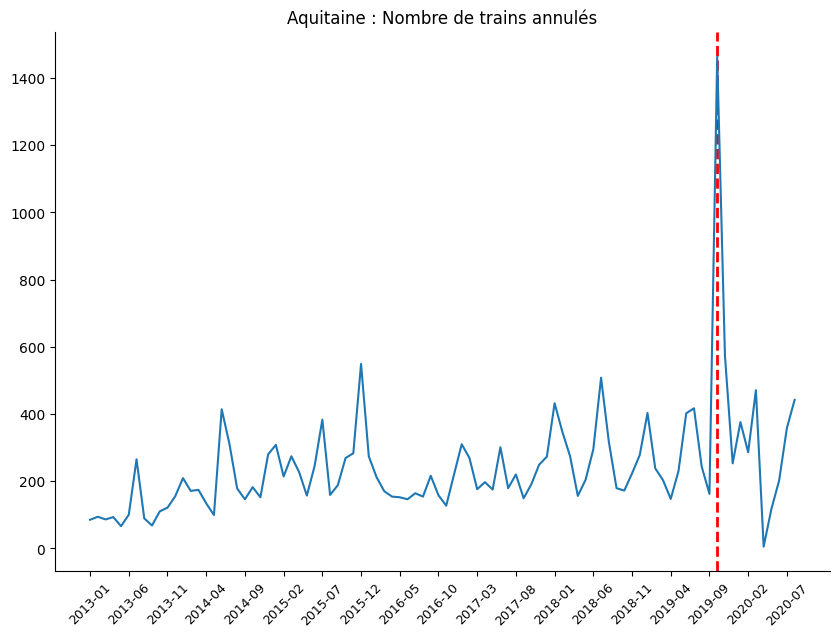
\includegraphics[width=0.8\textwidth]{image/AQ-FIG10.png} 
\caption{La date de repture.}
\label{fig:trains_ANNULES_2}
\end{figure}




\subsubsection{Test de Kolmogorov-Smirnov}

Nous appliquons le test de Kolmogorov-Smirnov aux deux échantillons. Nous obtenons \textbf{p-value= 0.03042677774966097 }: nous rejetons $H_0$.

\subsubsection{Évaluation des paramètres des lois}


$\hat{\mu_1}^k$,$\hat{\mu_2}^k$,$\hat{\sigma_1}^k$,$\hat{\sigma_2}^k$,$\hat{\theta}^k$=( 98.60025567  39.88619881 155.60519799 515.51660342   4.87537057)\\

Nous observons que la moyenne du nombre de trains annulés dans la région Aquitaine avant le point de rupture ($\hat{\mu_1}^k$) est supérieure à celle observée après le point de rupture ($\hat{\mu_2}^k$), révélant ainsi une diminution du nombre moyen de trains annulés post-rupture. Par ailleurs, l'augmentation considérable de la variance après le point de rupture ($\hat{\sigma_2}^k$ en comparaison à $\hat{\sigma_1}^k$) indique une variabilité plus importante dans le nombre de trains annulés après cette date. Le paramètre de skewness positif ($\hat{\theta}^k$) suggère une asymétrie dans la distribution, avec une queue s'étendant plus significativement vers la droite. Cette asymétrie est illustrée par la Figure 3.46, où le trait rouge en pointillé marque un changement significatif dans la distribution des annulations de trains à l'instant de la rupture.


Ci-dessous, nous comparons les histogrammes des deux échantillons aux lois théoriques (\textit{cf Figures 3.35 et 3.36})

\begin{figure}[H]
  \centering
  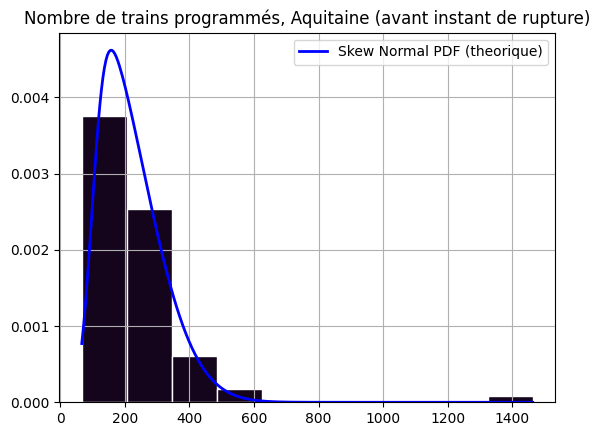
\includegraphics[width=0.7\textwidth]{image/AQ-FIG11.png}
  \caption{Histogramme de l'échantillon avant point de rupture}
\end{figure}

\begin{figure}[H]
  \centering
  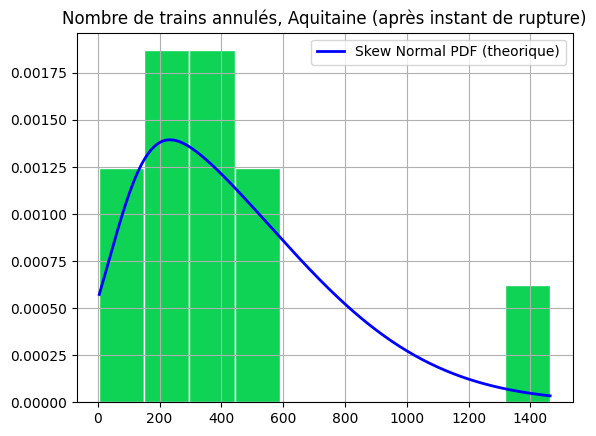
\includegraphics[width=0.7\textwidth]{image/AQ-FIG12.png}
  \caption{Histogramme de l'échantillon après point de rupture}
\end{figure}

Nous avons obtenu un paramètre $\hat{\theta}^k$ positif, ce qui indique des distributions normales asymétriques avec une queue plus étendue vers la droite pour la région Aquitaine. Cette caractéristique est clairement observée dans les histogrammes, tant pour l'échantillon avant qu'après le point de rupture. Les histogrammes révèlent une prévalence de valeurs excédant la moyenne sur le côté droit de la distribution, cohérente avec une skewness positive. Cette asymétrie dans la distribution du nombre de trains annulés est confirmée visuellement par les Figures 3.47 et 3.48, mettant en évidence une distribution qui penche davantage vers des valeurs supérieures après le point de rupture.



\section{Provence Alpes Côte d'Azur}

\subsection{Trains programmés}

\begin{figure}[H]
  \centering
  \includegraphics[width=0.7\textwidth]{PACA_TP_1.png}
  \caption{Nombre de trains programmés entre 01/2013 et 02/2024}
\end{figure}

\begin{figure}[H]
  \centering
  \includegraphics[width=0.7\textwidth]{PACA_TP_2.png}
  \caption{Histogramme du nombre de trains programmés}
\end{figure}

Nous appliquons notre méthode de detection de point de rupture et nous obtenons les résultats suivants:

\subsubsection{Moment de rupture $\hat{k}$}

La date de rupture obtenue est: \textbf{2018-02}. 

\begin{figure}[H]
  \centering
  \includegraphics[width=0.8\textwidth]{PACA_TP_3.png}
  \caption{Date de rupture}
\end{figure}

\subsubsection{Test de Kolmogorov-Smirnov}

Nous appliquons le test de Kolmogorov-Smirnov aux deux échantillons. Nous obtenons \textbf{p-value= 2.30e-06}: nous rejetons $H_0$, ainsi le point de rupture est pertinent.

\subsubsection{Évaluation des paramètres des lois}

$\hat{\mu_1}^k$,$\hat{\mu_2}^k$,$\hat{\sigma_1}^k$,$\hat{\sigma_2}^k$,$\hat{\theta}^k$=(15925.16, 15384.91,  2025.92,  3341.31, -4657.06)\\

Nous constatons que la moyenne de la loi normale asymétrique avant point de rupture est légèrement plus élevée que pour celle après point de rupture. Mais surtout, nous observons une augmentation significante de la variance apès point de rupture. Ces observations sont cohérentes avec ce que nous observons à la \textit{Figure 3.51}.\\


Ci-dessous, nous comparons les histogrammes des deux échantillons aux lois théoriques (\textit{cf Figures 3.52 et 3.53})

\begin{figure}[H]
  \centering
  \includegraphics[width=0.7\textwidth]{PACA_TP_4.png}
  \caption{Histogramme de l'échantillon avant point de rupture}
\end{figure}

\begin{figure}[H]
  \centering
  \includegraphics[width=0.7\textwidth]{PACA_TP_5.png}
  \caption{Histogramme de l'échantillon après point de rupture}
\end{figure}

Nous avions obtenu un paramètre $\hat{\theta}^k$ négatif, c'est à dire des lois normales asymétriques pour lesquelles la distribution est inclinée vers la droite, avec une queue de distribution plus importante sur la gauche. Cela parait cohérent avec les histogrammes obtenus.\\
En revanche, la correspondance entre droite théorique et histogramme est un peu décevante, en particulier pour la Figure 3.9.

\subsection{Trains annulés}

\begin{figure}[H]
  \centering
  \includegraphics[width=0.7\textwidth]{PACA_TA_1.png}
  \caption{Nombre de trains annulés entre 01/2013 et 02/2024}
\end{figure}

\begin{figure}[H]
  \centering
  \includegraphics[width=0.7\textwidth]{PACA_TA_2.png}
  \caption{Histogramme du nombre de trains annulés}
\end{figure}

Nous appliquons notre méthode de detection de point de rupture et nous obtenons les résultats suivants:

\subsubsection{Moment de rupture $\hat{k}$}

La date de rupture obtenue est: \textbf{2014-02}. 

\begin{figure}[H]
  \centering
  \includegraphics[width=0.7\textwidth]{PACA_TA_3_bis.png}
  \caption{Recherche du moment de rupture optimal}
\end{figure}

\begin{figure}[H]
  \centering
  \includegraphics[width=0.7\textwidth]{PACA_TA_3.png}
  \caption{Date de rupture}
\end{figure}

\subsubsection{Test de Kolmogorov-Smirnov}

Nous appliquons le test de Kolmogorov-Smirnov aux deux échantillons. Nous obtenons \textbf{p-value= 9.50e-05}: nous rejetons $H_0$, ainsi le point de rupture est pertinent.
\subsubsection{Évaluation des paramètres des lois}

$\hat{\mu_1}^k$,$\hat{\mu_2}^k$,$\hat{\sigma_1}^k$,$\hat{\sigma_2}^k$,$\hat{\theta}^k$=(285.35, 238.41, 1052.41, 294.60, 3.03)\\

Comme précédemment la moyenne de la loi normale asymétrique avant point de rupture est légèrement plus élevée que celle après point de rupture. Le changement le plus important concerne les variances: la variance de la loi normale assymétrique avant rupture est bien plus élevée comparée à la varaince de la loi normale assymétrique après rupture. Ces observations sont cohérentes avec ce que nous observons à la \textit{Figure 3.57}.\\

Ci-dessous, nous comparons les histogrammes des deux échantillons aux lois théoriques (\textit{cf Figures 3.58 et 3.59})

\begin{figure}[H]
  \centering
  \includegraphics[width=0.7\textwidth]{PACA_TA_4.png}
  \caption{Histogramme de l'échantillon avant point de rupture}
\end{figure}

\begin{figure}[H]
  \centering
  \includegraphics[width=0.7\textwidth]{PACA_TA_5.png}
  \caption{Histogramme de l'échantillon après point de rupture}
\end{figure}

Nous avions obtenu un paramètre $\hat{\theta}^k$ positif, c'est à dire des lois normales asymétriques pour lesquelles la distribution est inclinée vers la gauche, avec une queue de distribution plus importante sur la droite. Cela parait cohérent avec les histogrammes obtenus. Puisque $\hat{\theta}^k$ est petit en valeur absolue, cela signifie que l'assymétrie est légère. C'est cohérent avec l'histogramme de l'échantillon après rupture mais pas très cohérent avec l'histogramme de l'échantillon avant rupture pour lequel l'assymétrie semble beaucoup plus prononcée. Dans ce cas, un modèle de rupture pour lequel les deux lois normales assymétriques ont chacune un paramètre ${\theta}$ différent aurait pu être plus adapté. \\

La correspondance entre droite théorique et histogramme est un peu décevante pour le figure avant rupture (\textit{cf Figure 3.58}). En revanche elle est satisfaisante pour la figure après rupture (\textit{cf Figure 3.59}).


\section{Normandie}

\subsection{Trains programmés}

\begin{figure}[H]
  \centering
  \includegraphics[width=0.7\textwidth]{Nor_TP_1.png}
  \caption{Nombre de trains programmés entre 01/2018 et 02/2024}
\end{figure}

\begin{figure}[H]
  \centering
  \includegraphics[width=0.7\textwidth]{Nor_TP_2.png}
  \caption{Histogramme du nombre de trains programmés}
\end{figure}

Nous appliquons notre méthode de detection de point de rupture et nous obtenons les résultats suivants:


\subsubsection{Moment de rupture $\hat{k}$}

La date de rupture obtenue est: \textbf{2019-11}. 

\begin{figure}[H]
  \centering
  \includegraphics[width=0.8\textwidth]{Nor_TP_3.png}
  \caption{Date de rupture}
\end{figure}

\subsubsection{Test de Kolmogorov-Smirnov}

Nous appliquons le test de Kolmogorov-Smirnov aux deux échantillons. Nous obtenons \textbf{p-value= 9.50e-05}: nous rejetons $H_0$, ainsi le point de rupture est pertinent.

\subsubsection{Évaluation des paramètres des lois}

$\hat{\mu_1}^k$,$\hat{\mu_2}^k$,$\hat{\sigma_1}^k$,$\hat{\sigma_2}^k$,$\hat{\theta}^k$=(9076.73,11520.44,1373.40 ,2933.11,-5965.37)\\

Nous constatons une moyenne plus élevée pour la loi normale assymétrique après le point de rupture comparé à celle avant le point de rupture. Nous constatons aussi une augmentation importante de la variance après le point de rupture. Ces observations sont cohérentes avec ce que nous observons à la \textit{Figure 3.62}.\\

Ci-dessous, nous comparons les histogrammes des deux échantillons aux lois théoriques (\textit{cf Figures 3.63 et 3.64})

\begin{figure}[H]
  \centering
  \includegraphics[width=0.7\textwidth]{Nor_TP_4.png}
  \caption{Histogramme de l'échantillon avant point de rupture}
\end{figure}

\begin{figure}[H]
  \centering
  \includegraphics[width=0.7\textwidth]{Nor_TP_5.png}
  \caption{Histogramme de l'échantillon après point de rupture}
\end{figure}

Nous avions obtenu un paramètre $\hat{\theta}^k$ négatif, c'est à dire des lois normales asymétriques pour lesquelles la distribution est inclinée vers la droite, avec une queue de distribution plus importante sur la gauche. Puisque $\hat{\theta}^k$ est grand en valeur absolue, cela signifie que l'assymétrie est importante. Cela parait cohérent avec les histogrammes obtenus.\\
En revanche, la correspondance entre droite théorique et histogramme est décevante.

\subsection{Trains annulés}

\begin{figure}[H]
  \centering
  \includegraphics[width=0.7\textwidth]{Nor_TA_1.png}
  \caption{Nombre de trains annulés entre 01/2018 et 02/2024}
\end{figure}

\begin{figure}[H]
  \centering
  \includegraphics[width=0.7\textwidth]{Nor_TA_2.png}
  \caption{Histogramme du nombre de trains annulés}
\end{figure}

Nous appliquons notre méthode de detection de point de rupture et nous obtenons les résultats suivants:

\subsubsection{Moment de rupture $\hat{k}$}

La date de rupture obtenue est: \textbf{2019-09}. 

\begin{figure}[H]
  \centering
  \includegraphics[width=0.7\textwidth]{Nor_TA_3_bis.png}
  \caption{Recherche du moment de rupture optimal}
\end{figure}

\begin{figure}[H]
  \centering
  \includegraphics[width=0.7\textwidth]{Nor_TA_3.png}
  \caption{Date de rupture}
\end{figure}

\subsubsection{Test de Kolmogorov-Smirnov}

Nous appliquons le test de Kolmogorov-Smirnov aux deux échantillons. Nous obtenons \textbf{p-value= 0.007}: nous rejetons $H_0$, ainsi le point de rupture est pertinent.
\subsubsection{Évaluation des paramètres des lois}

$\hat{\mu_1}^k$,$\hat{\mu_2}^k$,$\hat{\sigma_1}^k$,$\hat{\sigma_2}^k$,$\hat{\theta}^k$=(62.36,  52.55, 71.21, 170.25, 6.13)\\

La moyenne de la loi normale asymétrique avant point de rupture est plus élevée que celle après point de rupture. Le changement le plus important concerne les variances: la variance de la loi normale assymétrique après rupture est bien plus élevée que la variance de la loi normale assymétrique avant point rupture. Ces observations sont cohérentes avec ce que nous observons à la \textit{Figure 3.68}.\\

Ci-dessous, nous comparons les histogrammes des deux échantillons aux lois théoriques (\textit{cf Figures 3.69 et 3.70})

\begin{figure}[H]
  \centering
  \includegraphics[width=0.7\textwidth]{Nor_TA_4.png}
  \caption{Histogramme de l'échantillon avant point de rupture}
\end{figure}

\begin{figure}[H]
  \centering
  \includegraphics[width=0.7\textwidth]{Nor_TA_5.png}
  \caption{Histogramme de l'échantillon après point de rupture}
\end{figure}

Nous avions obtenu un paramètre $\hat{\theta}^k$ positif, c'est à dire des lois normales asymétriques pour lesquelles la distribution est inclinée vers la gauche, avec une queue de distribution plus importante sur la droite. Puisque $\hat{\theta}^k$ est petit en valeur absolue, cela signifie que l'assymétrie est légère. Cela parait cohérent avec les histogrammes obtenus.

La correspondance entre droite théorique et histogramme est satisfaisante pour les deux échantillons.

\section{Hauts-de-France}

\subsection{Trains programmés}

\begin{figure}[H]
  \centering
  \includegraphics[width=0.7\textwidth]{HF_TP_1.png}
  \caption{Nombre de trains programmés entre 01/2018 et 02/2024}
\end{figure}

\begin{figure}[H]
  \centering
  \includegraphics[width=0.7\textwidth]{HF_TP_2.png}
  \caption{Histogramme du nombre de trains programmés}
\end{figure}

Nous appliquons notre méthode de detection de point de rupture et nous obtenons les résultats suivants:

\subsubsection{Moment de rupture $\hat{k}$}

La date de rupture obtenue est: \textbf{2021-08}. 

\begin{figure}[H]
  \centering
  \includegraphics[width=0.8\textwidth]{HF_TP_3.png}
  \caption{Date de rupture}
\end{figure}

\subsubsection{Test de Kolmogorov-Smirnov}

Nous appliquons le test de Kolmogorov-Smirnov aux deux échantillons. Nous obtenons \textbf{p-value= 0.04}: nous rejetons $H_0$, ainsi le point de rupture est pertinent.\\

\\Cependant, nous remarquons que notre p-value est plutôt élevée comparé à ce que nous avions pû obtenir précédemment. Avec un niveau de confiance plus important (par exemple $\alpha$=0,01) nous n'aurions pas assez de preuve pour rejeter $H_0$

\subsubsection{Évaluation des paramètres des lois}

$\hat{\mu_1}^k$,$\hat{\mu_2}^k$,$\hat{\sigma_1}^k$,$\hat{\sigma_2}^k$,$\hat{\theta}^k$=(30788.67, 31398.90, 8249.20, 4146.03, -6679.83)\\

Nous constatons une hausse légère de la moyenne après le point de rupture. Mais de manière plus significative, nous observons que la variance de la loi avant point de rupture est le double de celle de la loi après point de rupture. Ces observations sont cohérentes avec ce que nous observons à la \textit{Figure 3.73}.\\

Ci-dessous, nous comparons les histogrammes des deux échantillons aux lois théoriques (\textit{cf Figures 3.74 et 3.75})

\begin{figure}[H]
  \centering
  \includegraphics[width=0.7\textwidth]{HF_TP_4.png}
  \caption{Histogramme de l'échantillon avant point de rupture}
\end{figure}

\begin{figure}[H]
  \centering
  \includegraphics[width=0.7\textwidth]{HF_TP_5.png}
  \caption{Histogramme de l'échantillon après point de rupture}
\end{figure}

Nous avions obtenu un paramètre $\hat{\theta}^k$ négatif, c'est à dire des lois normales asymétriques pour lesquelles la distribution est inclinée vers la droite, avec une queue de distribution plus importante sur la gauche. Cela parait cohérent avec les histogrammes obtenus.
En revanche, la correspondance entre droite théorique et histogramme est un peu décevante, particulièrement pour la Figure 3.74.

\subsection{Trains annulés}

\begin{figure}[H]
  \centering
  \includegraphics[width=0.7\textwidth]{HF_TA_1.png}
  \caption{Nombre de trains annulés entre 01/2018 et 02/2024}
\end{figure}

\begin{figure}[H]
  \centering
  \includegraphics[width=0.7\textwidth]{HF_TA_2.png}
  \caption{Histogramme du nombre de trains annulés}
\end{figure}

Nous appliquons notre méthode de detection de point de rupture et nous obtenons les résultats suivants:

\subsubsection{Moment de rupture $\hat{k}$}

La date de rupture obtenue est: \textbf{2020-01}. 

\begin{figure}[H]
  \centering
  \includegraphics[width=0.7\textwidth]{HF_TA_3_bis.png}
  \caption{Recherche du moment de rupture optimal}
\end{figure}

\begin{figure}[H]
  \centering
  \includegraphics[width=0.7\textwidth]{HF_TA_3.png}
  \caption{Date de rupture}
\end{figure}

\subsubsection{Test de Kolmogorov-Smirnov}

Nous appliquons le test de Kolmogorov-Smirnov aux deux échantillons. Nous obtenons \textbf{p-value= 1.90e-05}: nous rejetons $H_0$, ainsi le point de rupture est pertinent.

\subsubsection{Évaluation des paramètres des lois}

$\hat{\mu_1}^k$,$\hat{\mu_2}^k$,$\hat{\sigma_1}^k$,$\hat{\sigma_2}^k$,$\hat{\theta}^k$=(405.98, 438.87, 223.43, 718.55, 2.68)\\

Nous constatons une augmentation de la moyenne après le moment de rupture. De même, la variance augmente après la rupture mais de manière plus impotante. Ces observations sont cohérentes avec ce que nous observons à la \textit{Figure 3.79}.\\

Ci-dessous, nous comparons les histogrammes des deux échantillons aux lois théoriques (\textit{cf Figures 3.80 et 3.81})

\begin{figure}[H]
  \centering
  \includegraphics[width=0.7\textwidth]{HF_TA_4.png}
  \caption{Histogramme de l'échantillon avant point de rupture}
\end{figure}

\begin{figure}[H]
  \centering
  \includegraphics[width=0.7\textwidth]{HF_TA_5.png}
  \caption{Histogramme de l'échantillon après point de rupture}
\end{figure}

Nous avions obtenu un paramètre $\hat{\theta}^k$ positif, c'est à dire des lois normales asymétriques pour lesquelles la distribution est inclinée vers la gauche, avec une queue de distribution plus importante sur la droite.Cela parait cohérent avec les histogrammes obtenus. 

En revanche, la correspondance entre droite théorique et histogramme est un peu décevante.

\section{Auverge-Rhône-Alpes}


\subsection{Trains programmés}

\begin{figure}[H]
  \centering
  \includegraphics[width=0.7\textwidth]{image/ARA_TP_1.png}
  \caption{Nombre de trains programmés entre 01/2018 et 02/2024}
\end{figure}

\begin{figure}[H]
  \centering
  \includegraphics[width=0.7\textwidth]{image/ARA_TP_2.png}
  \caption{Histogramme du nombre de trains programmés}
\end{figure}

Nous appliquons notre méthode de detection de point de rupture et nous obtenons les résultats suivants:

\subsubsection{Moment de rupture $\hat{k}$}

La date de rupture obtenue est: \textbf{2021-09}. 

\begin{figure}[H]
  \centering
  \includegraphics[width=0.8\textwidth]{image/ARA_TP_3.png}
  \caption{Date de rupture}
\end{figure}

\subsubsection{Test de Kolmogorov-Smirnov}

Nous appliquons le test de Kolmogorov-Smirnov aux deux échantillons. Nous obtenons \textbf{p-value=  4.36-11}: nous rejetons $H_0$, ainsi le point de rupture est pertinent.

\subsubsection{Évaluation des paramètres des lois}

$\hat{\mu_1}^k$,$\hat{\mu_2}^k$,$\hat{\sigma_1}^k$,$\hat{\sigma_2}^k$,$\hat{\theta}^k$=(35702.70, 39669.58, 9849.48, 4294.28, -6.04)\\

Nous constatons que la moyenne de la loi normale asymétrique après le point de rupture est  plus élevée que pour celle avant point de rupture.De plus, nous observons une baisse importante de la variance après point de rupture. Ces observations sont cohérentes avec ce que nous observons à la \textit{Figure 3.84}.\\


Ci-dessous, nous comparons les histogrammes des deux échantillons aux lois théoriques (\textit{cf Figures 3.85 et 3.86})

\begin{figure}[H]
  \centering
  \includegraphics[width=0.7\textwidth]{image/ARA_TP_4.png}
  \caption{Histogramme de l'échantillon avant point de rupture}
\end{figure}

\begin{figure}[H]
  \centering
  \includegraphics[width=0.7\textwidth]{image/ARA_TP_5.png}
  \caption{Histogramme de l'échantillon après point de rupture}
\end{figure}

Nous avions obtenu un paramètre $\hat{\theta}^k$ négatif, c'est à dire des lois normales asymétriques pour lesquelles la distribution est inclinée vers la droite, avec une queue de distribution plus importante sur la gauche. Cela parait cohérent avec les histogrammes obtenus.\\

En revanche, la correspondance entre droite théorique et histogramme est un peu décevante.

\subsection{Trains annulés}

\begin{figure}[H]
  \centering
  \includegraphics[width=0.7\textwidth]{image/ARA_TA_1.png}
  \caption{Nombre de trains annulés entre 01/2018 et 02/2024}
\end{figure}

\begin{figure}[H]
  \centering
  \includegraphics[width=0.7\textwidth]{image/ARA_TA_2.png}
  \caption{Histogramme du nombre de trains annulés}
\end{figure}

Nous appliquons notre méthode de detection de point de rupture et nous obtenons les résultats suivants:

\subsubsection{Moment de rupture $\hat{k}$}

La date de rupture obtenue est: \textbf{2020-06}. 

\begin{figure}[H]
  \centering
  \includegraphics[width=0.7\textwidth]{image/ARA_TA_3_bis.png}
  \caption{Recherche du moment de rupture optimal}
\end{figure}

\begin{figure}[H]
  \centering
  \includegraphics[width=0.7\textwidth]{image/ARA_TA_3.png}
  \caption{Date de rupture}
\end{figure}

\subsubsection{Test de Kolmogorov-Smirnov}

Nous appliquons le test de Kolmogorov-Smirnov aux deux échantillons. Nous obtenons \textbf{p-value= 7.61e-05}: nous rejetons $H_0$, ainsi le point de rupture est pertinent.

\subsubsection{Évaluation des paramètres des lois}

$\hat{\mu_1}^k$,$\hat{\mu_2}^k$,$\hat{\sigma_1}^k$,$\hat{\sigma_2}^k$,$\hat{\theta}^k$=(180.63, 508.59, 490.83, 327.96, 4.58)\\

Nous constatons que la moyenne de la loi normale asymétrique après le point de rupture augmente tandis que la variance baisse. Cela parait cohérent avec ce que nous observons à la \textit{Figure 3.90}.\\

Ci-dessous, nous comparons les histogrammes des deux échantillons aux lois théoriques (\textit{cf Figures 3.91 et 3.92})

\begin{figure}[H]
  \centering
  \includegraphics[width=0.7\textwidth]{image/ARA_TA_4.png}
  \caption{Histogramme de l'échantillon avant point de rupture}
\end{figure}

\begin{figure}[H]
  \centering
  \includegraphics[width=0.7\textwidth]{image/ARA_TA_5.png}
  \caption{Histogramme de l'échantillon après point de rupture}
\end{figure}

Nous avions obtenu un paramètre $\hat{\theta}^k$ positif, c'est à dire des lois normales asymétriques pour lesquelles la distribution est inclinée vers la gauche, avec une queue de distribution plus importante sur la droite. Cela parait cohérent avec les histogrammes obtenus. \\

En outre, la correspondance entre droite théorique et histogramme est satisfaisante pour les deux échantillons.

}
\include{conclusion}

\renewcommand{\refname}{Biliographie}
\bibliographystyle{unsrt}
\bibliography{bib}\addcontentsline{toc}{chapter}{Bibliographie}

%\include{bibliographie}
%\include{abstract}
%\pagestyle{plain}
%\include{Annexe1}

% Fin du document
\end{document}
